\documentclass[14pt,a4paper]{extreport}

\usepackage{style/style}
\usepackage{physics}
\usepackage{fancyhdr}

\fancypagestyle{plain}{%
\fancyhf{} % clear all header and footer fields
\fancyfoot[C]{\small\thepage}}
\renewcommand{\headrulewidth}{0pt}
\renewcommand{\footrulewidth}{0pt}
\pagestyle{plain}

\makeatletter
  \def\my@tag@font{\small}
  \def\maketag@@@#1{\hbox{\m@th\normalfont\my@tag@font#1}}
  \let\amsmath@eqref\eqref
  \renewcommand\eqref[1]{{\let\my@tag@font\relax\amsmath@eqref{#1}}}
\makeatother

\usepackage{titletoc}
\titlecontents{chapter}[0em]{\bfseries}{\thecontentslabel.\hspace{1em}}{}{\titlerule*[1pc]{.}\contentspage}
\titlecontents{section}[1.25em]{}{\thecontentslabel.\hspace{1em}}{}{\titlerule*[1pc]{.}\contentspage}
\titlecontents{subsection}[2.5em]{}{\thecontentslabel.\hspace{1em}}{}{\titlerule*[1pc]{.}\contentspage}

\begin{document}

% Отключение нумерации страниц
\pagenumbering{gobble}

%\chapter*{Аннотация}

Отчёт 91 с., 4 ч., 24 рис., 26 табл., 13 источников, 1 прил.

ЧИСЛЕННОЕ МОДЕЛИРОВАНИЕ ЭЛЕКТРОМАГНИТНОГО \\ ПОЛЯ, МЕТОД КОНЕЧНЫХ ЭЛЕМЕНТОВ, МНОГОЭТАПНАЯ СХЕМА РАЗДЕЛЕНИЯ ПОЛЕЙ

Цель работы: разработка программы для численного моделирования нестационарного электромагнитного поля в трёхмерной среде, создаваемого индукционным источником тока, при помощи многоэтапной схемы разделения полей.

В процессе работы был разработан и протестирован  программный модуль численного моделирования электромагнитного поля с помощью многоэтапной схемы разделения полей.

С помощью программы проводилось исследование поведения поля в приповерхностных слоях земной коры с различными значениями удельной электропроводности горизонтально-слоистой среды и аномальных объектов. 

\newpage

\tableofcontents
\newpage

% Включение нумерации страниц
\pagenumbering{arabic}
\setcounter{page}{3}
\chapter*{Введение}

\addcontentsline{toc}{chapter}{Введение}

Под векторными задачами мы будем понимать задачи, в которых решением является некоторая вектор-функция. Будем рассматривать такие векторные задачи, решениями которых являются вектор-функции с компонентами, каждая из которых будет удовлетворять дифференциальному уравнению второго порядка и как минимум непрерывна. Таким образом, каждая из компонент искомой вектор-функции может быть найдена в виде линейной комбинации непрерывных базисных функции, которые использовались при решении скалярных задач. Такие базисные функции обычно называют узловыми (к ним относятся не только лагранжевы и эрмитовы базисные функции, но и иерархические). Соответственно и МКЭ, использующий при нахождении численного решения, такие базисные функции называют узловым.

Технологию построения конечноэлементных аппроксимации векторных задач на основе узлового МКЭ мы рассмотри на примере задачи (), описывающие нестационарное электромагнитное поле в однородной по магнитной проницаемости среде (и без учета токов смещения).
%\chapter{Исследования}

\section{Исследование первичного поля}

Пусть источник индукционного поля лежит на расстоянии $R = 500$ м от оси симметрии и имееет силу тока, равную $J_{\varphi} = 1.0$ А. Также условимся, что источник работал достаточно долго, чтобы создать стабильное электромагнитное поле. Сетка по времени равномерная: $t=[1.0; 1.05]$ на 200 временных слоёв. После истечения первой секунды мы отключим наш источник, т.е. $J_{\varphi} = 0.0$ A при $t > 1.0$. На рисунках \ref{fig:A_phi_0} -- \ref{fig:E_phi_2} представлено распространение этого поля в среде в начальный, промежуточных и последний момент времени.

\begin{figure}
	\centering
	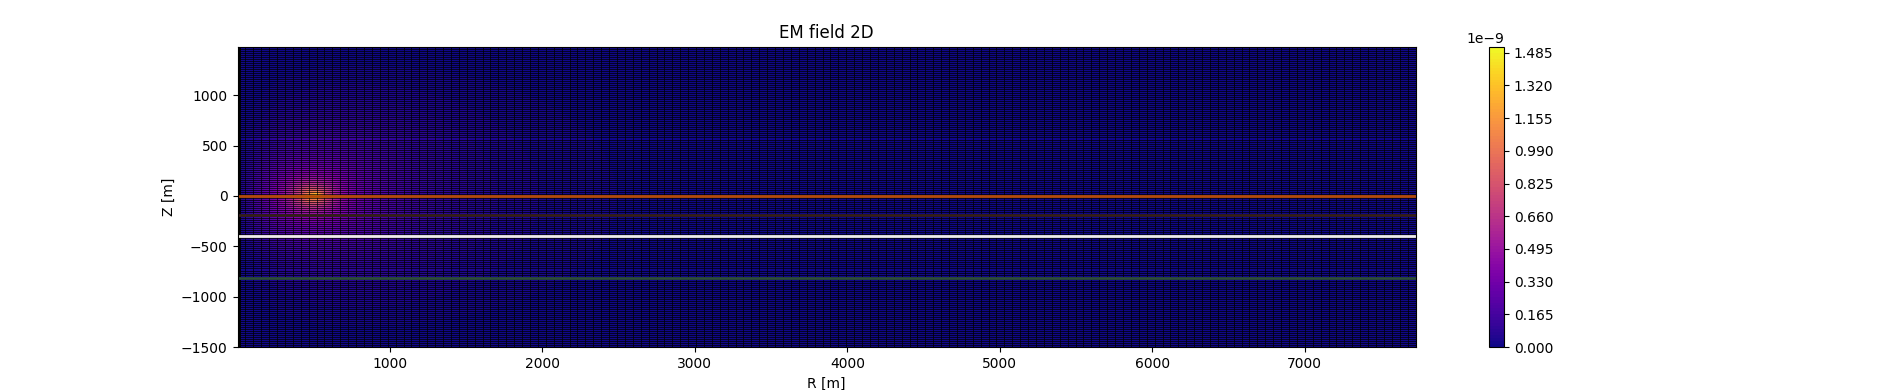
\includegraphics[width=1.0\linewidth]{images/Answer_A_time_layer_1.png}
	\caption{Решение $A_{\varphi}$ при $t = 1.0с$}
	\label{fig:A_phi_0}
\end{figure}

\begin{figure}
	\centering
	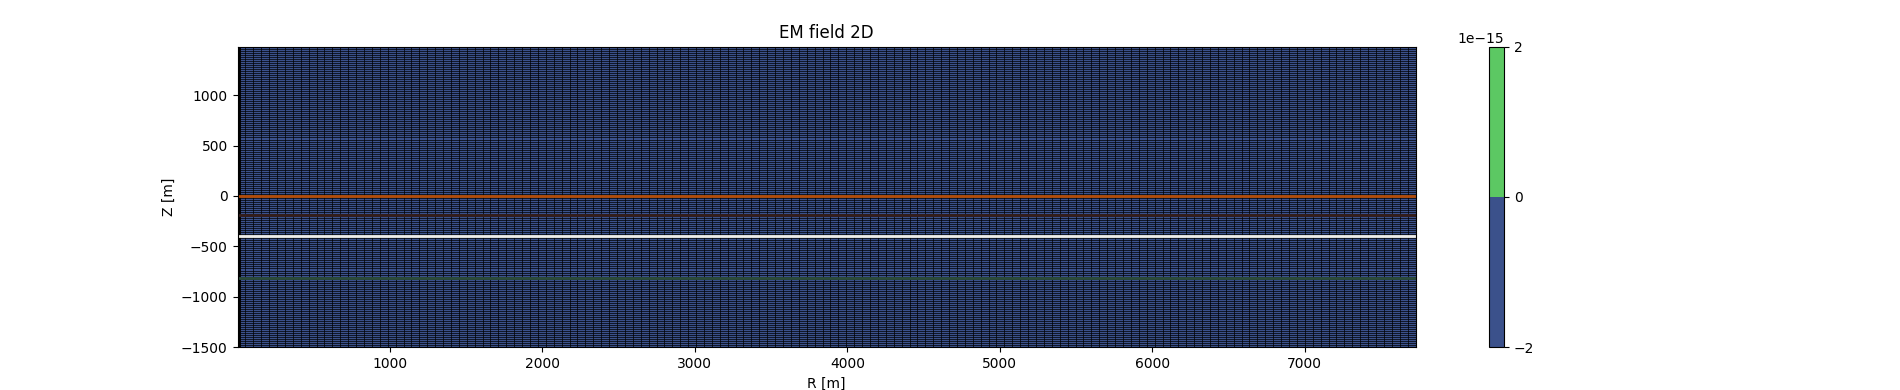
\includegraphics[width=1.0\linewidth]{images/Answer_E_time_layer_1.png}
	\caption{Решение $E_{\varphi}$ при $t = 1.0с$}
	\label{fig:E_phi_0}
\end{figure}

\begin{figure}
	\centering
	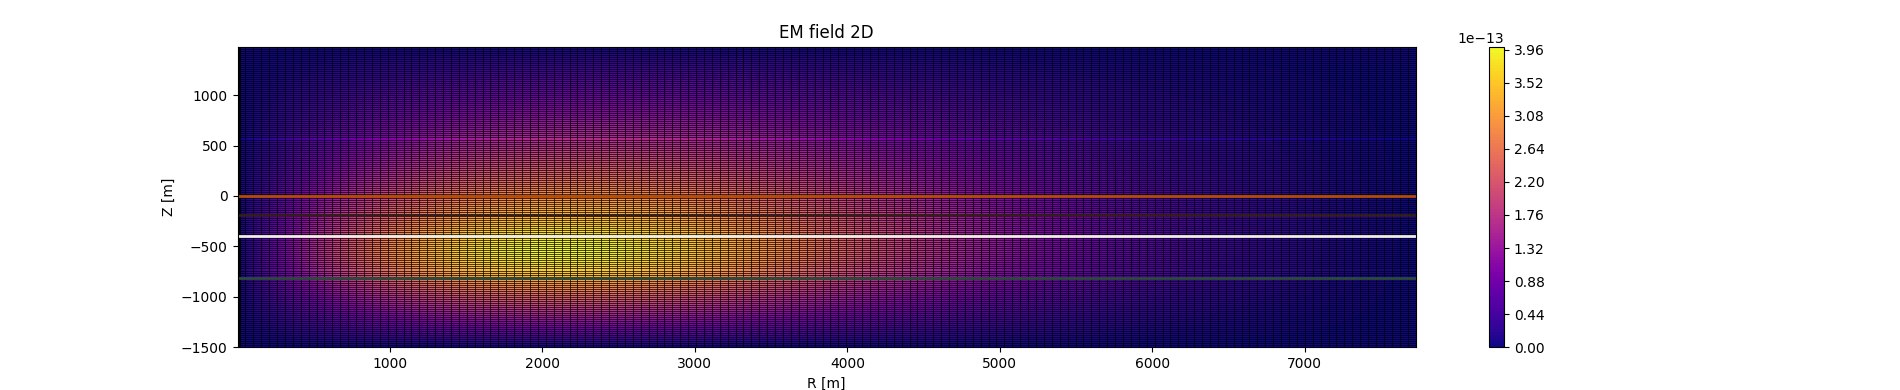
\includegraphics[width=1.0\linewidth]{images/Answer_A_time_layer_1.0250000000000083.png}
	\caption{Решение $A_{\varphi}$ при $t = 1.025с$}
	\label{fig:A_phi_1}
\end{figure}

\begin{figure}
	\centering
	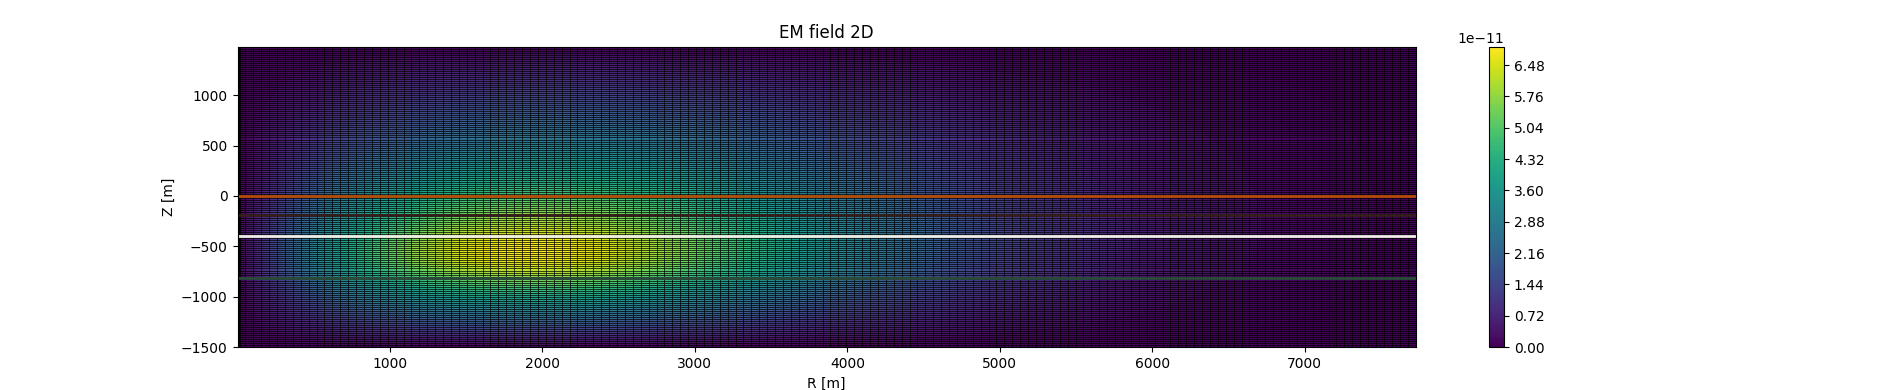
\includegraphics[width=1.0\linewidth]{images/Answer_E_time_layer_1.0250000000000083.png}
	\caption{Решение $E_{\varphi}$ при $t = 1.025с$}
	\label{fig:E_phi_1}
\end{figure} 

\begin{figure}
	\centering
	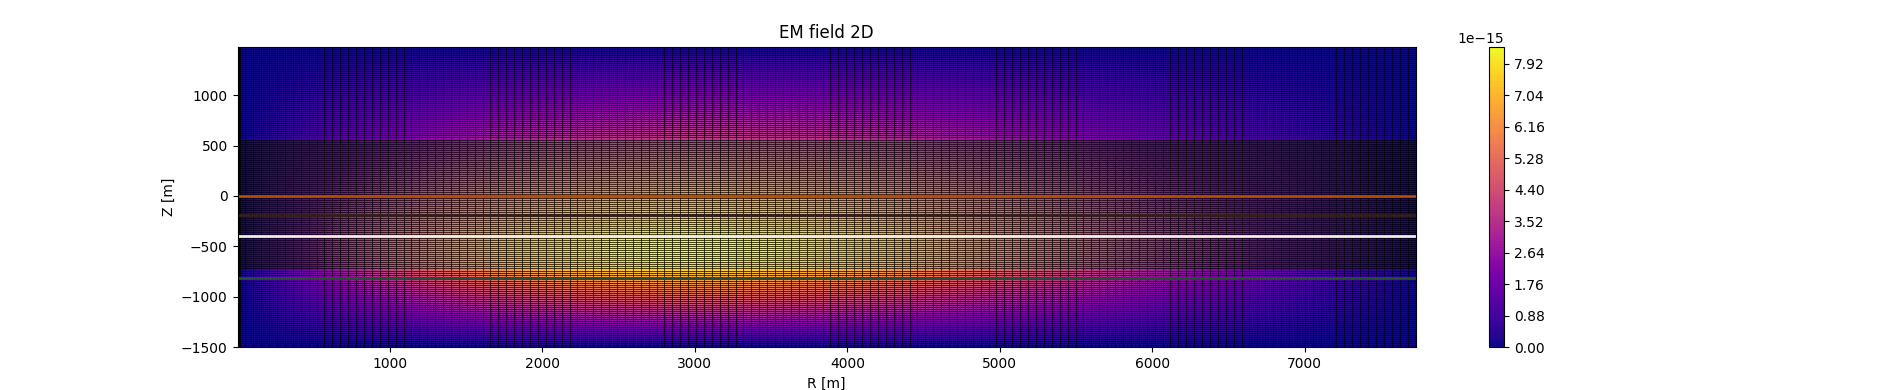
\includegraphics[width=1.0\linewidth]{images/Answer_A_time_layer_1.05.png}
	\caption{Решение $A_{\varphi}$ при $t = 1.05с$}
	\label{fig:A_phi_2}
\end{figure}

\begin{figure}
	\centering
	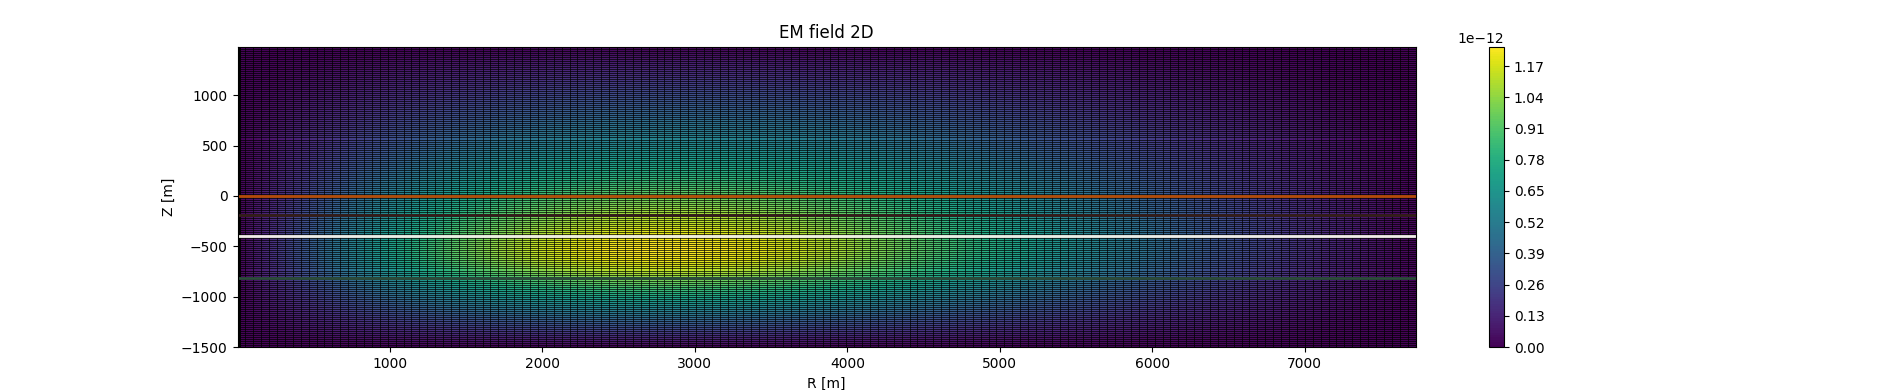
\includegraphics[width=1.0\linewidth]{images/Answer_E_time_layer_1.05.png}
	\caption{Решение $A_{\varphi}$ при $t = 1.05с$}
	\label{fig:E_phi_2}
\end{figure} 

Расположим на расчётной области приёмники в каждой горизонтально-слоистой среде и проведем замеры значений вектор-потенциала и электрического поля в точках $(2500; 0; -100)$, $(2500; 0; -200)$, $(10; 0; -700)$, $(1000; 0; -1250)$. Отобразим на графиках \ref{fig:NatA} -- \ref{fig:LogE} полученные значения.

\begin{figure}
	\centering
	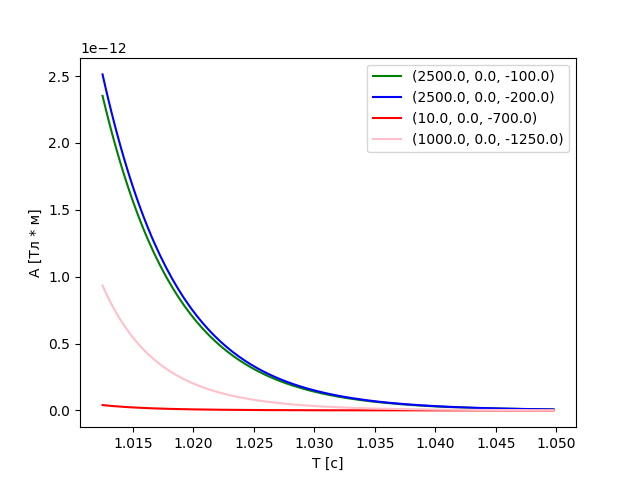
\includegraphics[width=0.8\linewidth]{images/Normal_A.png}
	\caption{Зависимость значения $A_{\varphi}$ от времени в разных приёмниках}
	\label{fig:NatA}
\end{figure}

\begin{figure}
	\centering
	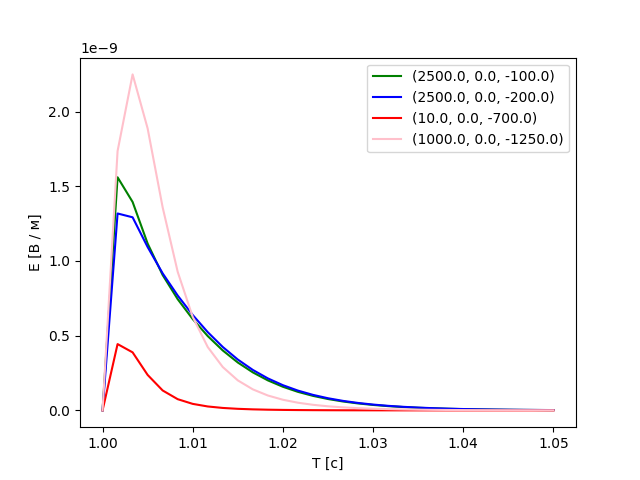
\includegraphics[width=0.8\linewidth]{images/Normal_E.png}
	\caption{Зависимость значения $E_{\varphi}$ от времени в разных приёмниках}
	\label{fig:NatE}
\end{figure}


\begin{figure}
	\centering
	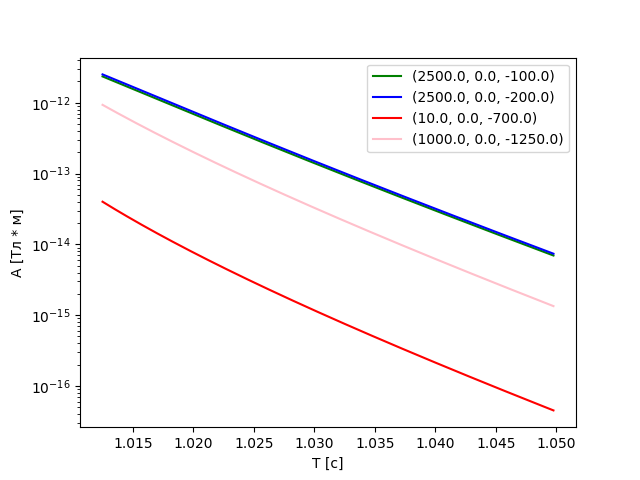
\includegraphics[width=0.8\linewidth]{images/Log_A.png}
	\caption{Зависимость значения $A_{\varphi}$ от времени в разных приёмниках (логарифмическая шкала по оси абсцисс)}
	\label{fig:LogA}
\end{figure}

\begin{figure}
	\centering
	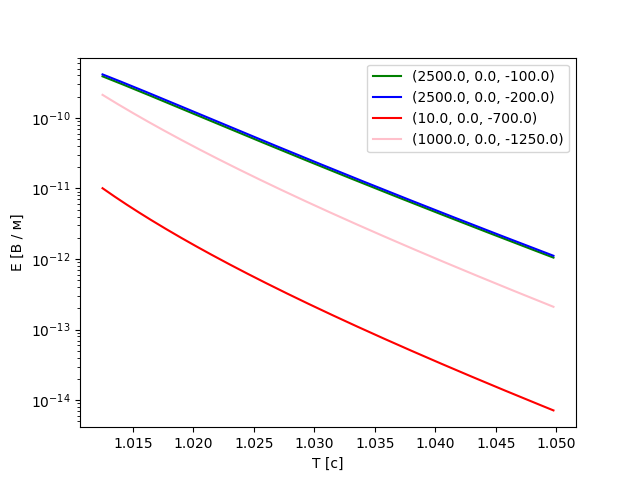
\includegraphics[width=0.8\linewidth]{images/Log_E.png}
	\caption{Зависимость значения $E_{\varphi}$ от времени в разных приёмниках (логарифмическая шкала по оси абсцисс)}
	\label{fig:LogE}
\end{figure} 

Как видим, значения вектор-потенциала и электрической напряжённости поля не имеют каких-либо резких колебаний. Из этого можно заключить, что, как и предполагалось, никаких аномальных зон в исследуемой области нет. 

\section{Исследование при разделении нормального и добавочного поля}

Добавим в нашу область аномальный объект со следующими границами: $[-5500; 5500]_x \times [2205; 2355]_y \times [-180; -80]_z$ и значением $\sigma = 4$. Будем искать решение из уравнения на добавочное поле (\ref{eq_1_6}). Получим решения изображенные на рисунках \ref{fig:A_plus_t0} -- \ref{fig:E_plus_t2}.

\begin{figure}
	\centering
	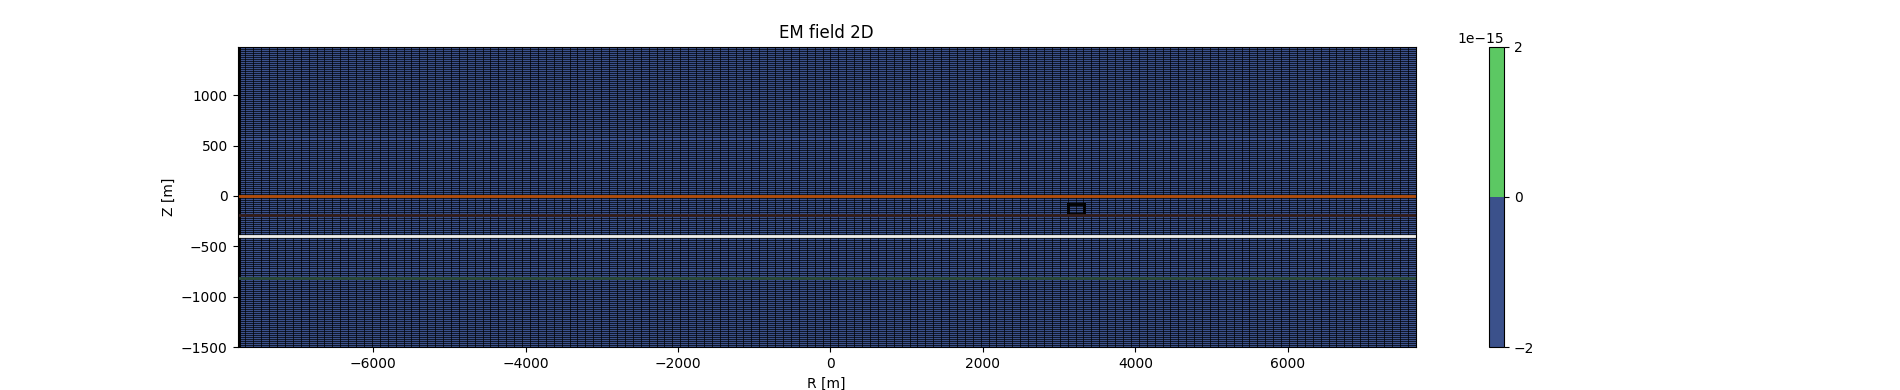
\includegraphics[width=1.0\linewidth]{images/Answer_A_plus_time_layer_1.png}
	\caption{Решение $\overrightarrow{\textbf{A}}^+$ при $t = 1.0с$}
	\label{fig:A_plus_t0}
\end{figure} 


\begin{figure}
	\centering
	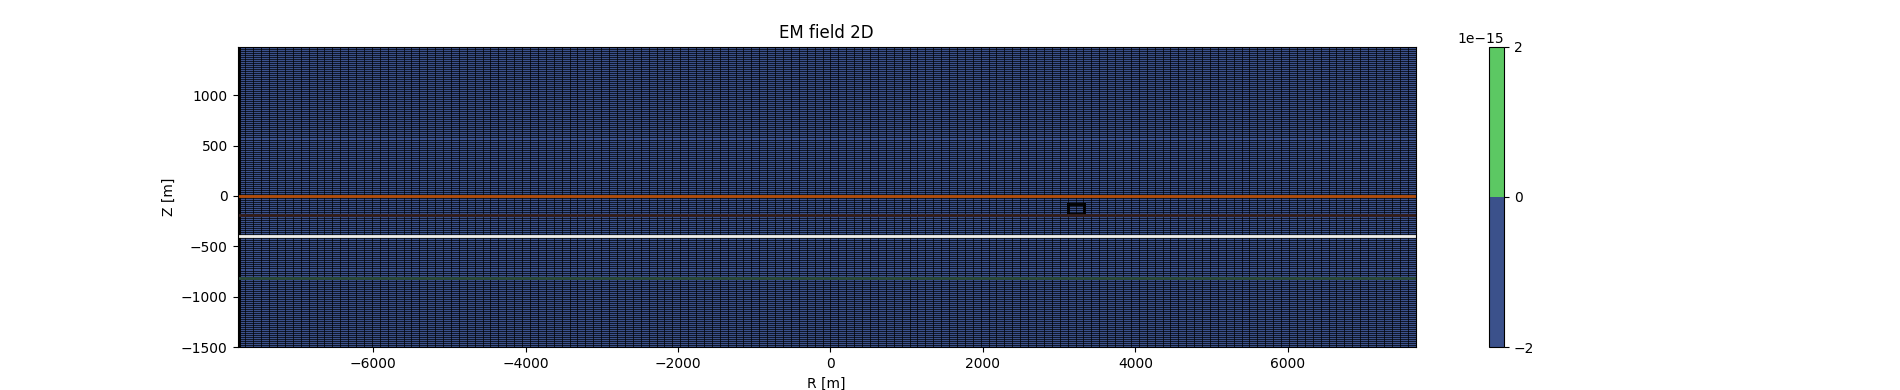
\includegraphics[width=1.0\linewidth]{images/Answer_E_plus_time_layer_1.png}
	\caption{Решение $\overrightarrow{\textbf{E}}^+$ при $t = 1.0с$}
	\label{fig:E_plus_t0}
\end{figure} 


\begin{figure}
	\centering
	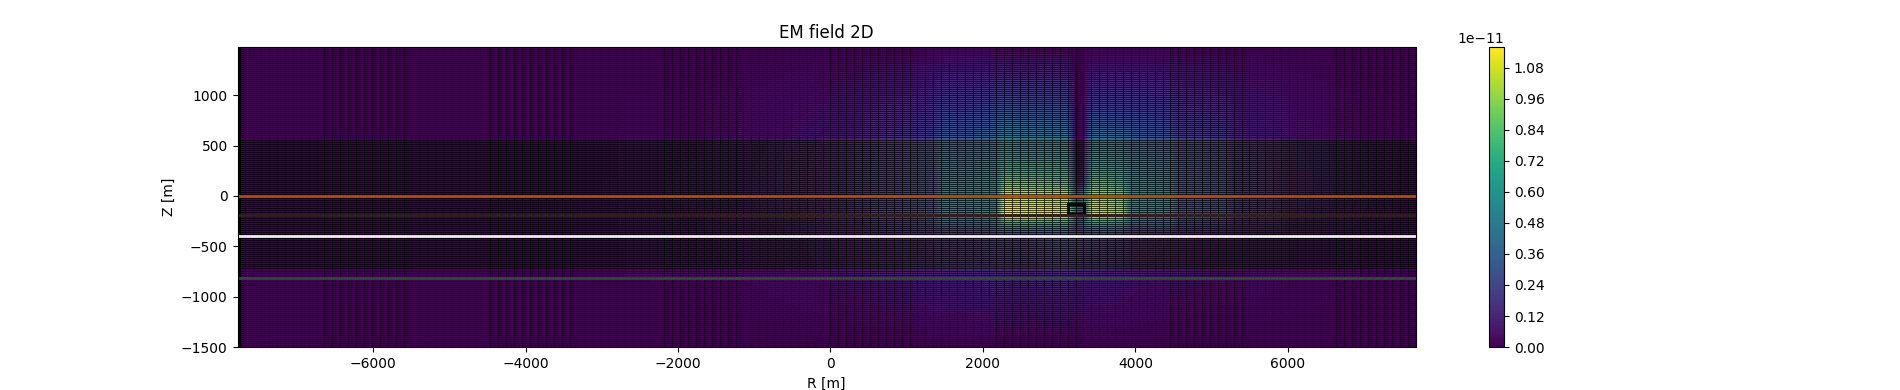
\includegraphics[width=1.0\linewidth]{images/Answer_A_plus_time_layer_1.0250000000000006.png}
	\caption{Решение $\overrightarrow{\textbf{A}}^+$ при $t = 1.025с$}
	\label{fig:A_plus_t1}
\end{figure} 


\begin{figure}
	\centering
	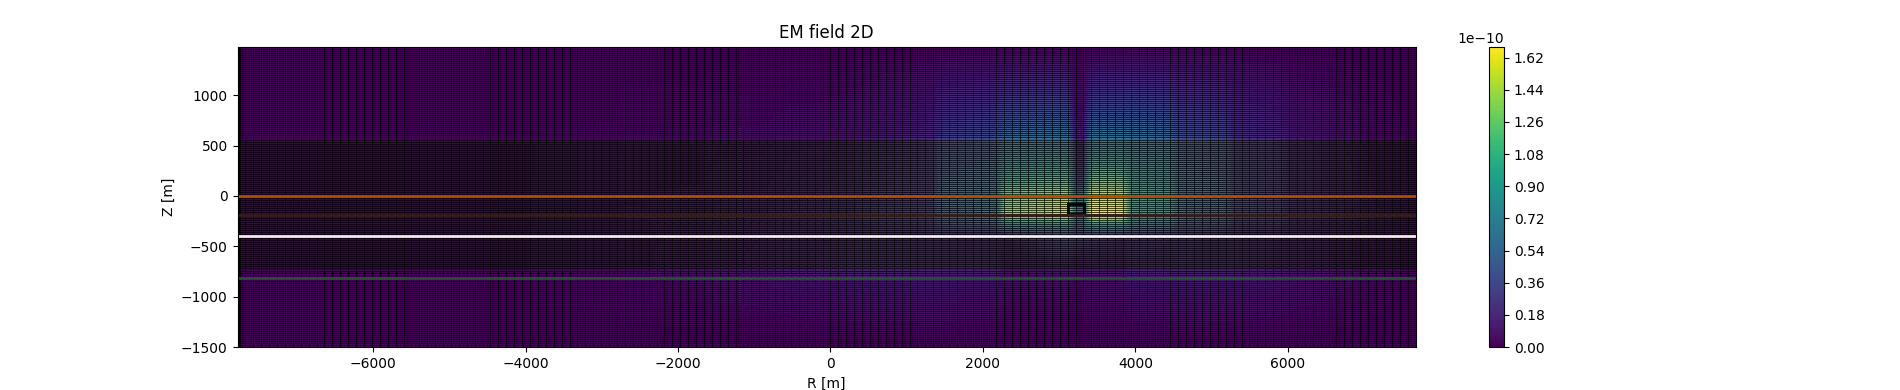
\includegraphics[width=1.0\linewidth]{images/Answer_E_plus_time_layer_1.0250000000000006.png}
	\caption{Решение $\overrightarrow{\textbf{E}}^+$ при $t = 1.025с$}
	\label{fig:E_plus_t1}
\end{figure} 

\begin{figure}
	\centering
	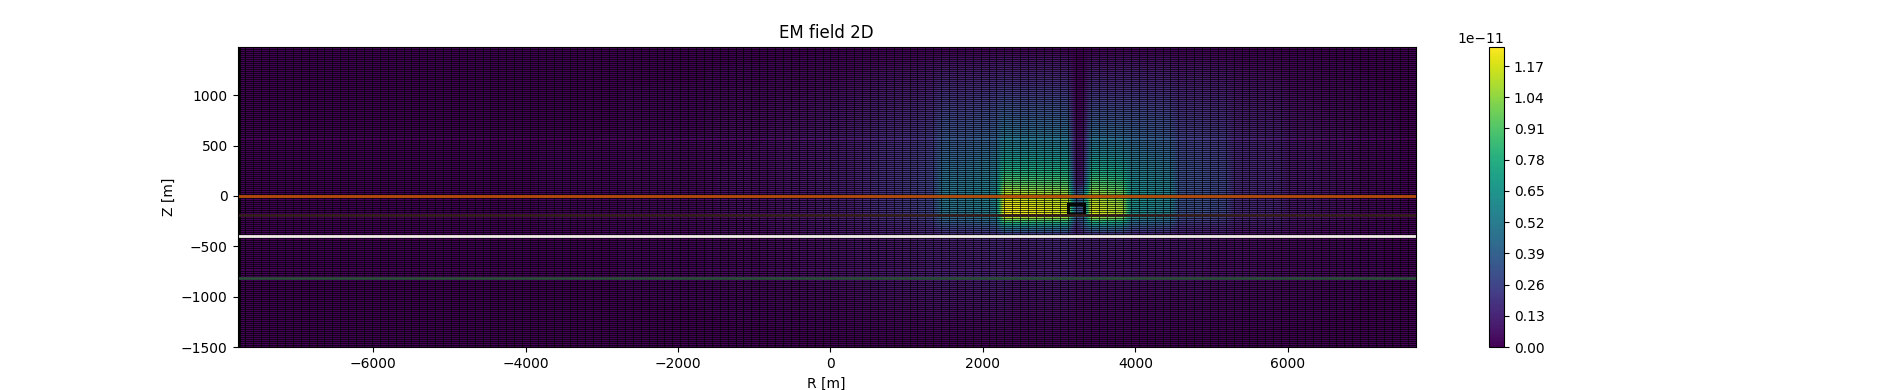
\includegraphics[width=1.0\linewidth]{images/Answer_A_plus_time_layer_1.05.png}
	\caption{Решение $\overrightarrow{\textbf{A}}^+$ при $t = 1.05с$}
	\label{fig:A_plus_t2}
\end{figure} 


\begin{figure}
	\centering
	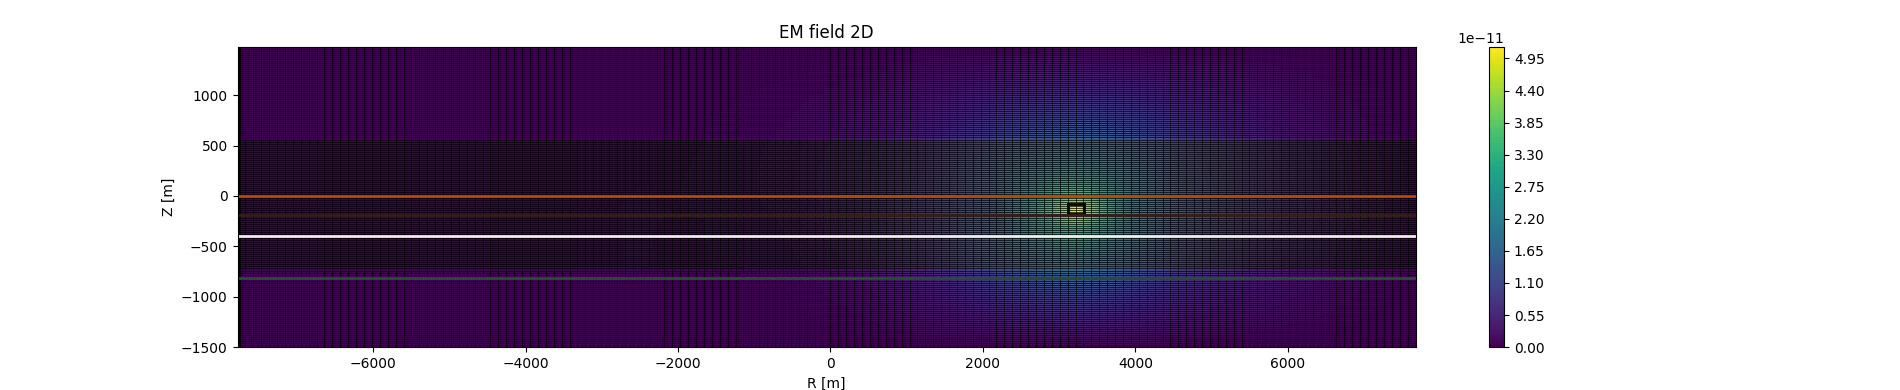
\includegraphics[width=1.0\linewidth]{images/Answer_E_plus_time_layer_1.05.png}
	\caption{Решение $\overrightarrow{\textbf{E}}^+$ при $t = 1.05с$}
	\label{fig:E_plus_t2}
\end{figure} 

Рассмотрим для $t = 1.0, t = 1.025, t = 1.05$ значения $\overrightarrow{\textbf{A}}^+$ и $\overrightarrow{\textbf{E}}^+$ на линии, перпендикулярно проходящей к аномальному объекту по оси $y$ при $x = 0.0, z = -130.0$. Получим следующее:

\begin{figure}
	\centering
	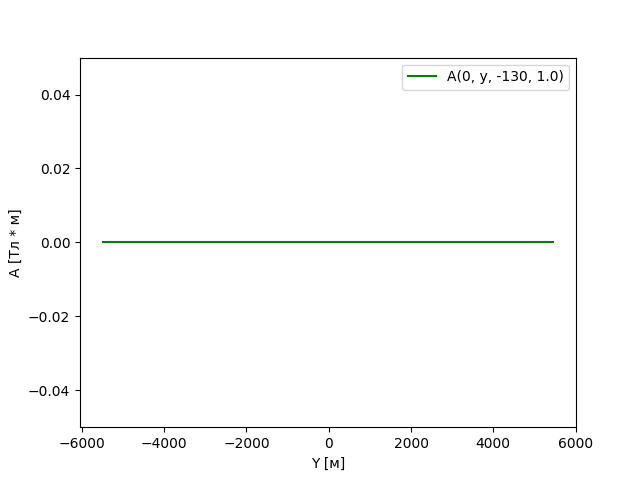
\includegraphics[width=0.5\linewidth]{images/Normal_A(y)_1.png}
	\caption{Решение $\overrightarrow{\textbf{A}}^+$ на линии $(0.0, y, -130.0)$ при $t = 1.0с$}
	\label{fig:A_line_t0}
\end{figure} 

\begin{figure}
	\centering
	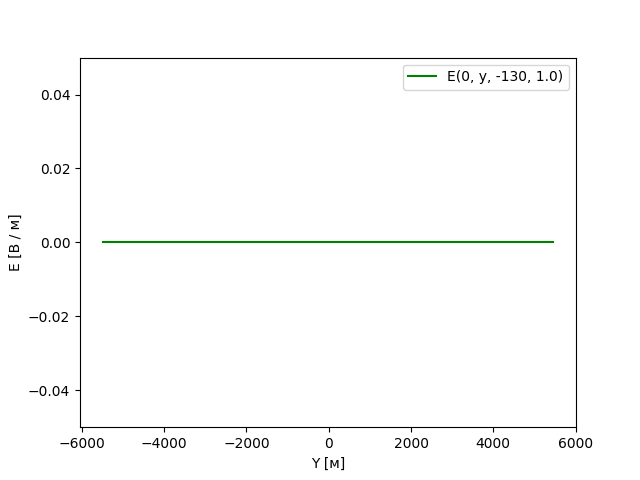
\includegraphics[width=0.5\linewidth]{images/Normal_E(y)_1.png}
	\caption{Решение $\overrightarrow{\textbf{E}}^+$ на линии $(0.0, y, -130.0)$ при $t = 1.0с$}
	\label{fig:E_line_t0}
\end{figure} 

\begin{figure}
	\centering
	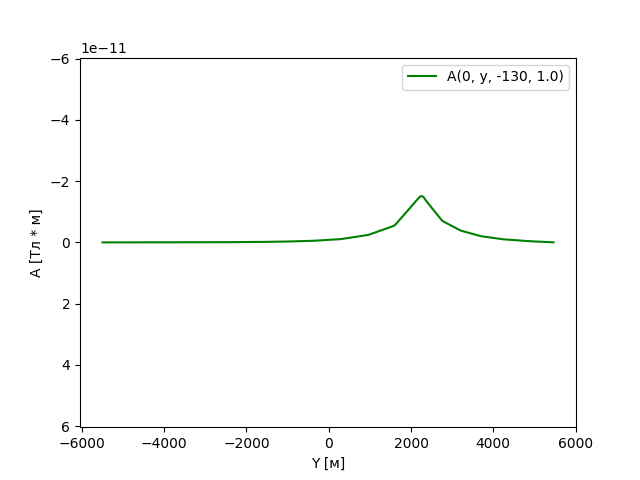
\includegraphics[width=0.5\linewidth]{images/Normal_A(y)_2.png}
	\caption{Решение $\overrightarrow{\textbf{A}}^+$ на линии $(0.0, y, -130.0)$ при $t = 1.025с$}
	\label{fig:A_line_t1}
\end{figure} 

\begin{figure}
	\centering
	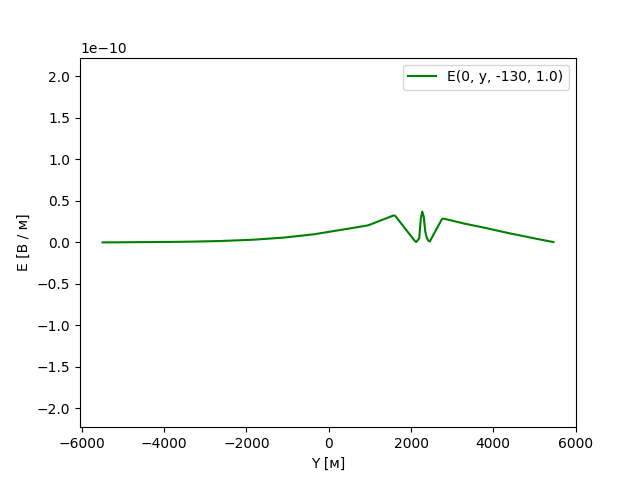
\includegraphics[width=0.5\linewidth]{images/Normal_E(y)_2.png}
	\caption{Решение $\overrightarrow{\textbf{E}}^+$ на линии $(0.0, y, -130.0)$  при $t = 1.025с$}
	\label{fig:E_line_t1}
\end{figure} 

\begin{figure}
	\centering
	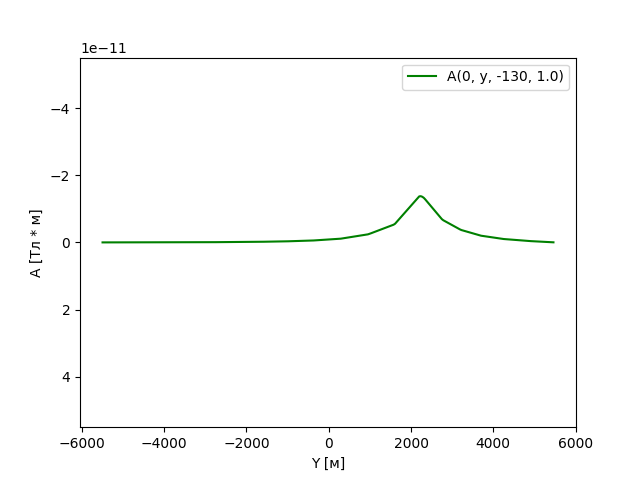
\includegraphics[width=0.5\linewidth]{images/Normal_A(y)_3.png}
	\caption{Решение $\overrightarrow{\textbf{A}}^+$ на линии $(0.0, y, -130.0)$  при $t = 1.05с$}
	\label{fig:A_line_t2}
\end{figure} 

\begin{figure}
	\centering
	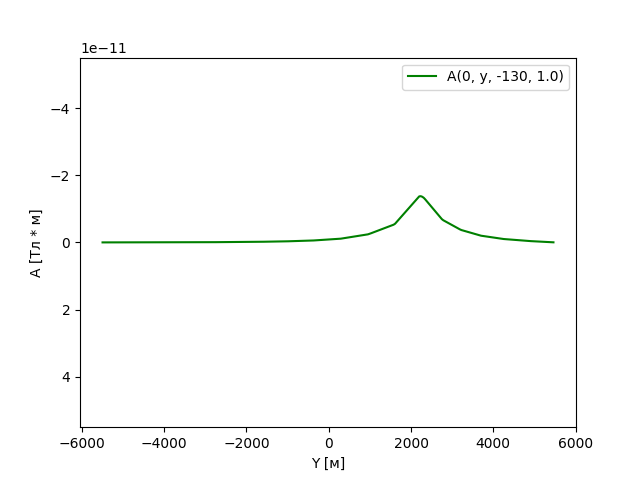
\includegraphics[width=0.5\linewidth]{images/Normal_A(y)_3.png}
	\caption{Решение $\overrightarrow{\textbf{A}}^+$ на линии $(0.0, y, -130.0)$  при $t = 1.05с$}
	\label{fig:E_line_t2}
\end{figure} 


Суммируем полученный результат с нормальным полем и получим состояние поля в разные моменты времени, изображённые на рисунках \ref{fig:A_Istage_t0} -- \ref{fig:E_Istage_t2}.

\begin{figure}
	\centering
	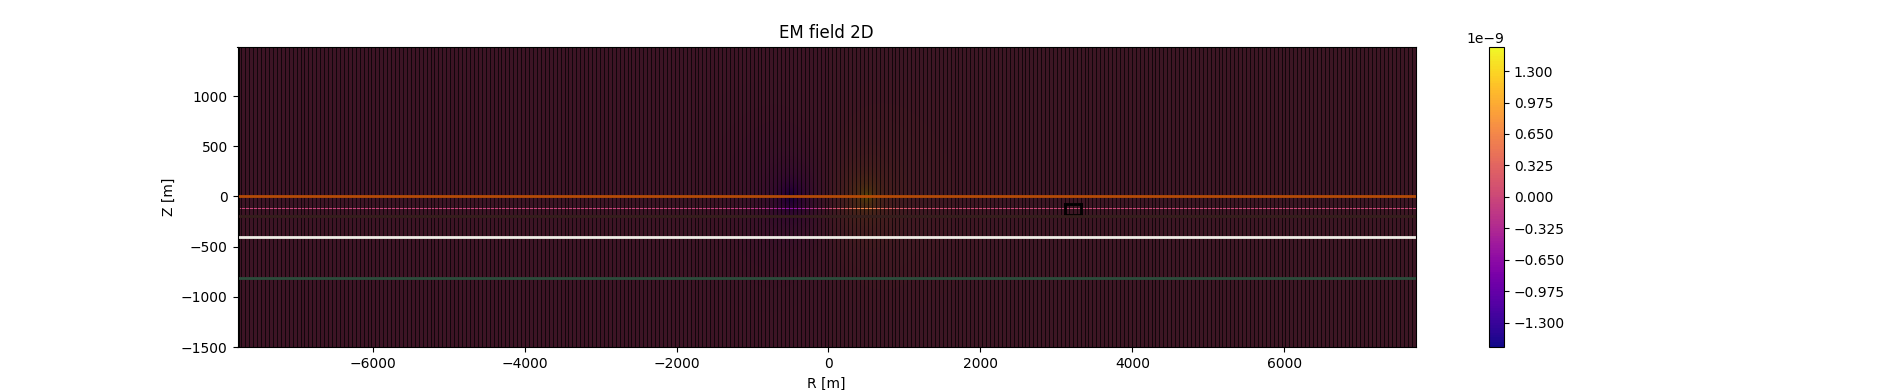
\includegraphics[width=1.0\linewidth]{images/Answer_A_Istage_time_layer_1.png}
	\caption{Решение суммарного поля $\overrightarrow{\textbf{A}}$ при $t = 1.0с$}
	\label{fig:A_Istage_t0}
\end{figure} 


\begin{figure}
	\centering
	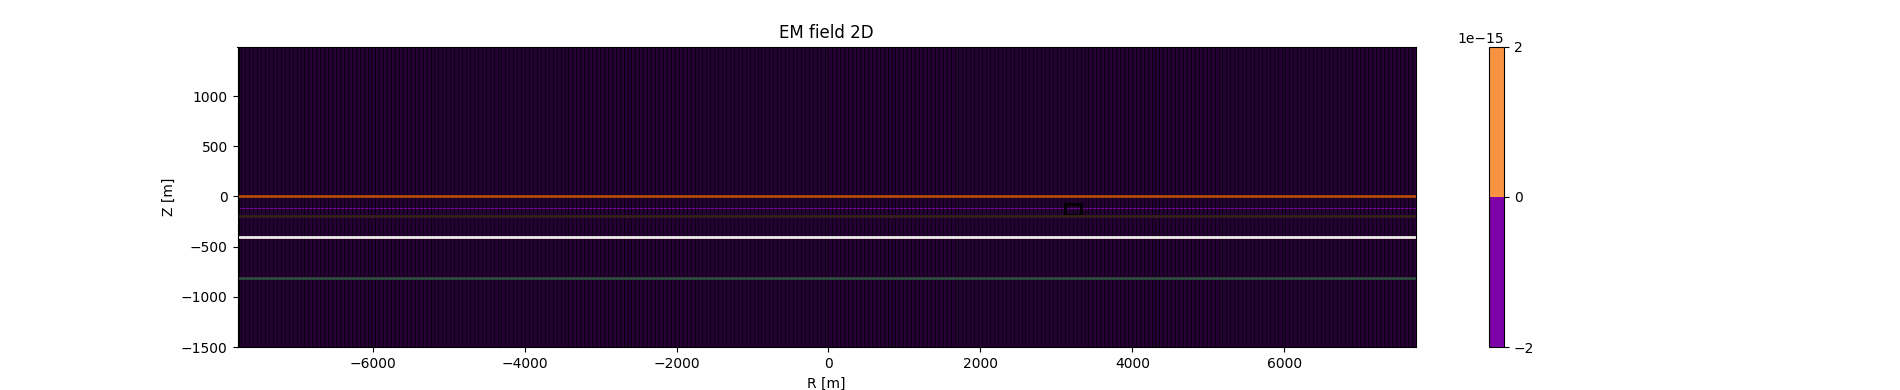
\includegraphics[width=1.0\linewidth]{images/Answer_E_Istage_time_layer_1.png}
	\caption{Решение суммарного поля $\overrightarrow{\textbf{E}}$ при $t = 1.0с$}
	\label{fig:E_Istage_t0}
\end{figure} 


\begin{figure}
	\centering
	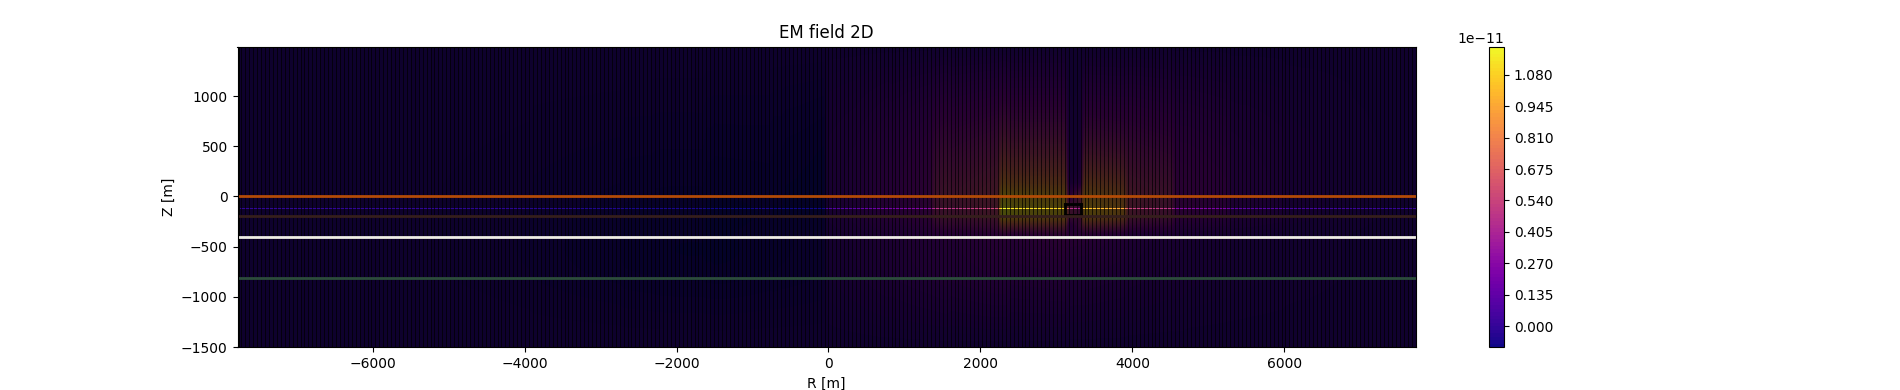
\includegraphics[width=1.0\linewidth]{images/Answer_A_Istage_time_layer_1.0250000000000006.png}
	\caption{Решение суммарного поля $\overrightarrow{\textbf{A}}$ при $t = 1.025с$}
	\label{fig:A_Istage_t1}
\end{figure} 


\begin{figure}
	\centering
	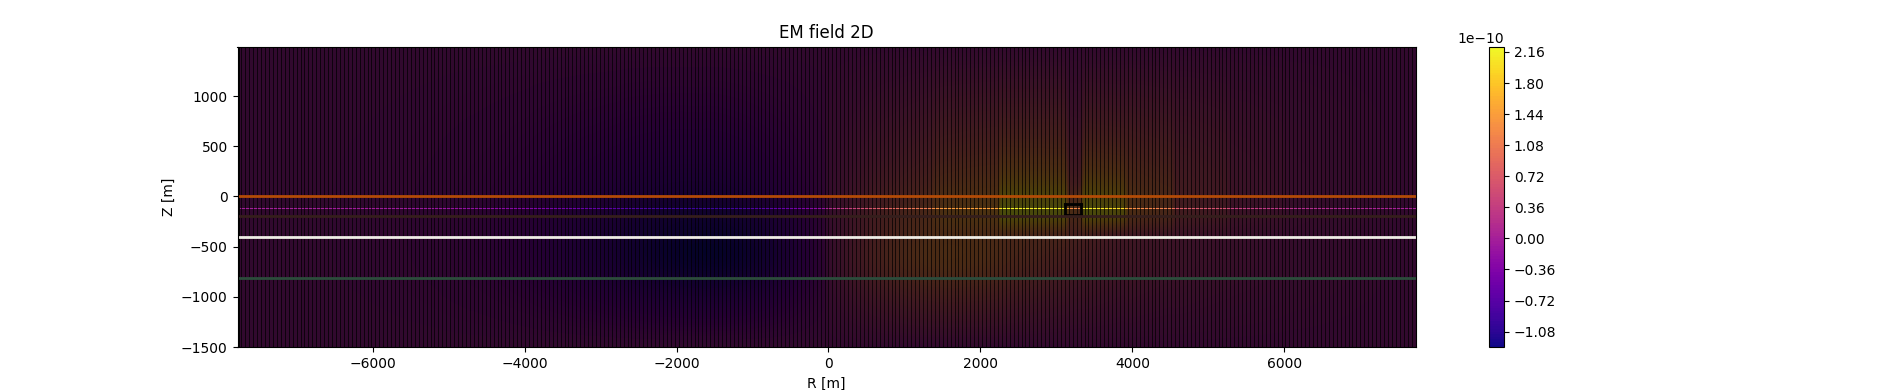
\includegraphics[width=1.0\linewidth]{images/Answer_E_Istage_time_layer_1.0250000000000006.png}
	\caption{Решение суммарного поля $\overrightarrow{\textbf{E}}$ при $t = 1.025с$}
	\label{fig:E_Istage_t1}
\end{figure} 

\begin{figure}
	\centering
	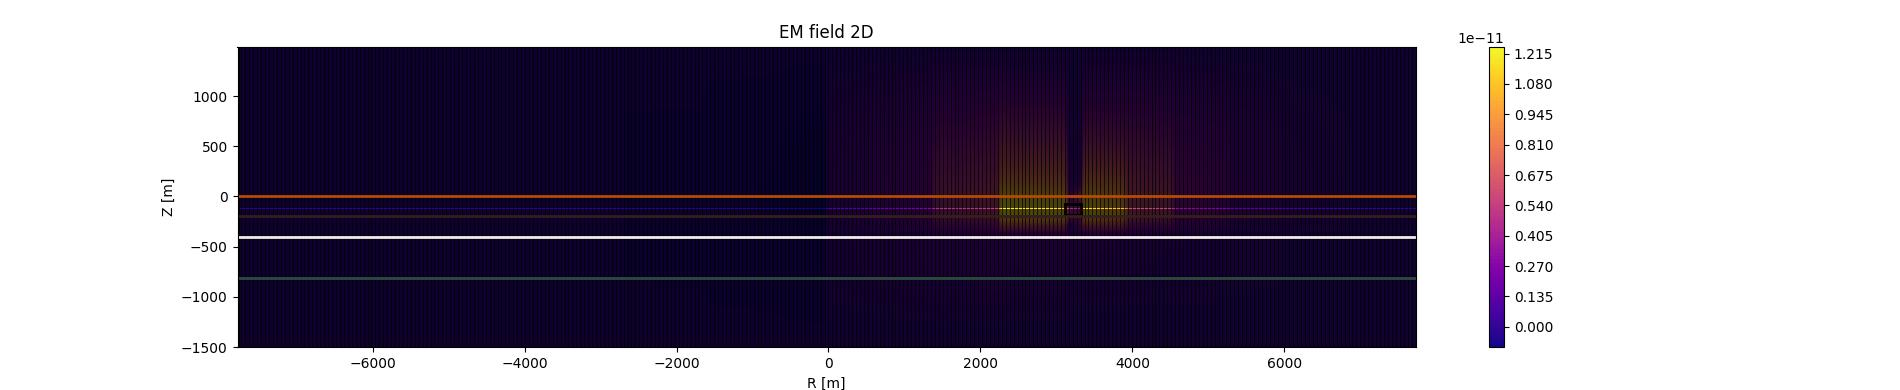
\includegraphics[width=1.0\linewidth]{images/Answer_A_Istage_time_layer_1.05.png}
	\caption{Решение суммарного поля $\overrightarrow{\textbf{A}}$ при $t = 1.05с$}
	\label{fig:A_Istage_t2}
\end{figure} 


\begin{figure}
	\centering
	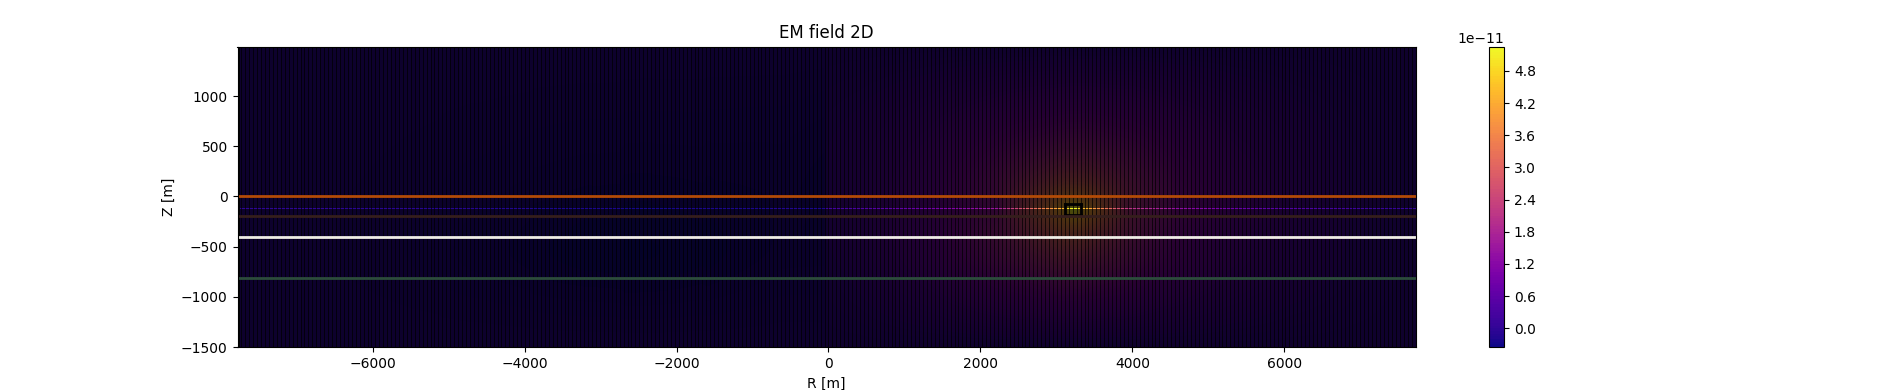
\includegraphics[width=1.0\linewidth]{images/Answer_E_Istage_time_layer_1.05.png}
	\caption{Решение суммарного поля $\overrightarrow{\textbf{E}}$ при $t = 1.05с$}
	\label{fig:E_Istage_t2}
\end{figure} 

Полученные значения \ref{fig:A_Log_added} -- \ref{fig:E_Log_added} $\overrightarrow{\textbf{A}}$ и $\overrightarrow{\textbf{E}}$ рассмотрим на приёмниках.

\begin{figure}
	\centering
	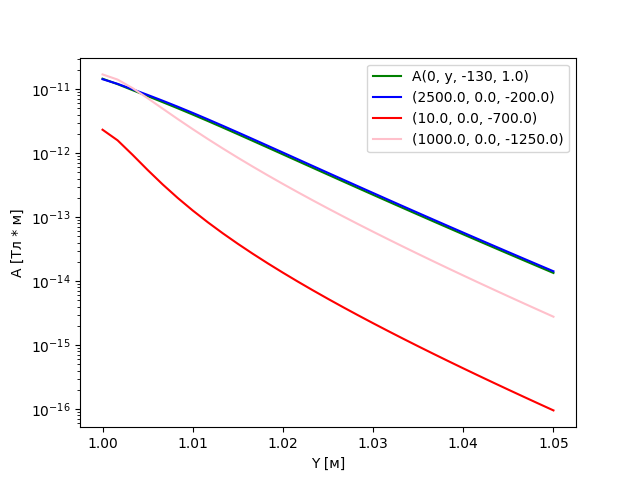
\includegraphics[width=0.8\linewidth]{images/Log_A_obj1.png}
	\caption{Решение суммарного поля $\overrightarrow{\textbf{E}}$ при $t = 1.05с$}
	\label{fig:A_Log_added}
\end{figure} 


\begin{figure}
	\centering
	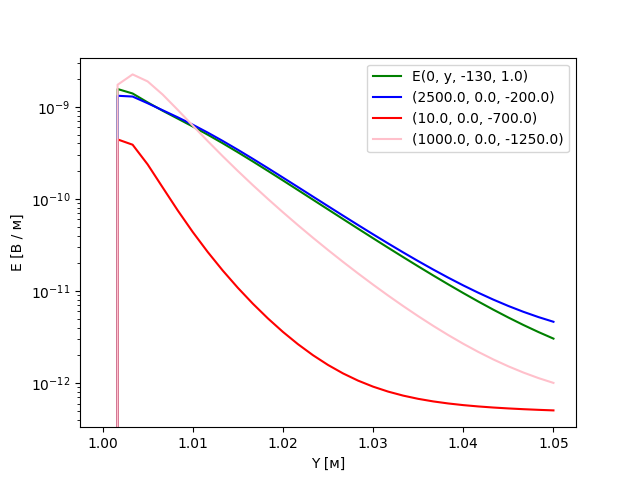
\includegraphics[width=0.8\linewidth]{images/Log_E_obj1.png}
	\caption{Решение суммарного поля $\overrightarrow{\textbf{E}}$ при $t = 1.05с$}
	\label{fig:E_Log_added}
\end{figure} 

Сравнивая показатели на приёмниках до добавления аномалии \ref{fig:LogA} -- \ref{fig:LogE} и после \ref{fig:A_Log_added} -- \ref{fig:A_Log_added}, можно заметить, что значения напряжённости электрического поля на красном приёмнике претерпели наиболее сильные изменения, т.к. он стал более похожим на гиперболу, нежели прямую линию. Значения на синем приёмнике начали изменяться уже в последние сотые секунды исследования. 

\section{Исследование многоэтапного разделения нормального и добавочных полей}

Добавим ещё один аномальный объект со следующими границами: $[-1305; -1050]_x \times [-2255; -2178]_y \times [-1250; -800]_z$ и значением $\sigma = 17$. Будем искать решение из уравнения на добавочное поле (\ref{eq_1_6}). Получим решения в разные моменты времени изображенные на рисунках \ref{fig:A_2plus_t0} -- \ref{fig:E_2plus_t2}.

\begin{figure}
	\centering
	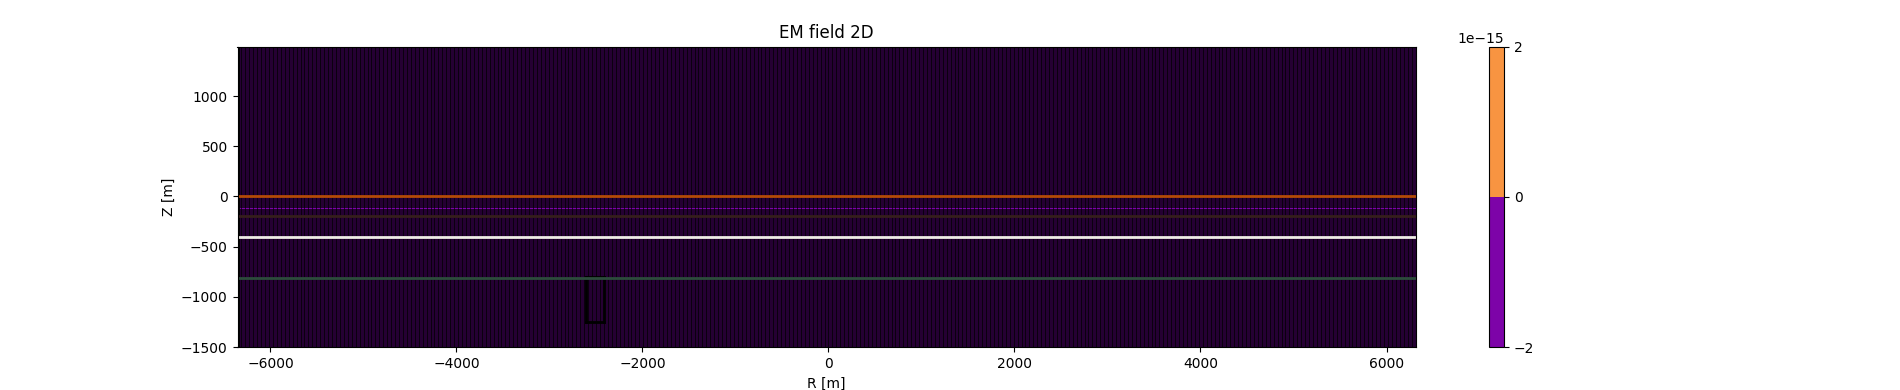
\includegraphics[width=1.0\linewidth]{images/Answer_A_2plus_time_layer_1.png}
	\caption{Решение $\overrightarrow{\textbf{A}}^+$ при $t = 1.0с$}
	\label{fig:A_2plus_t0}
\end{figure} 


\begin{figure}
	\centering
	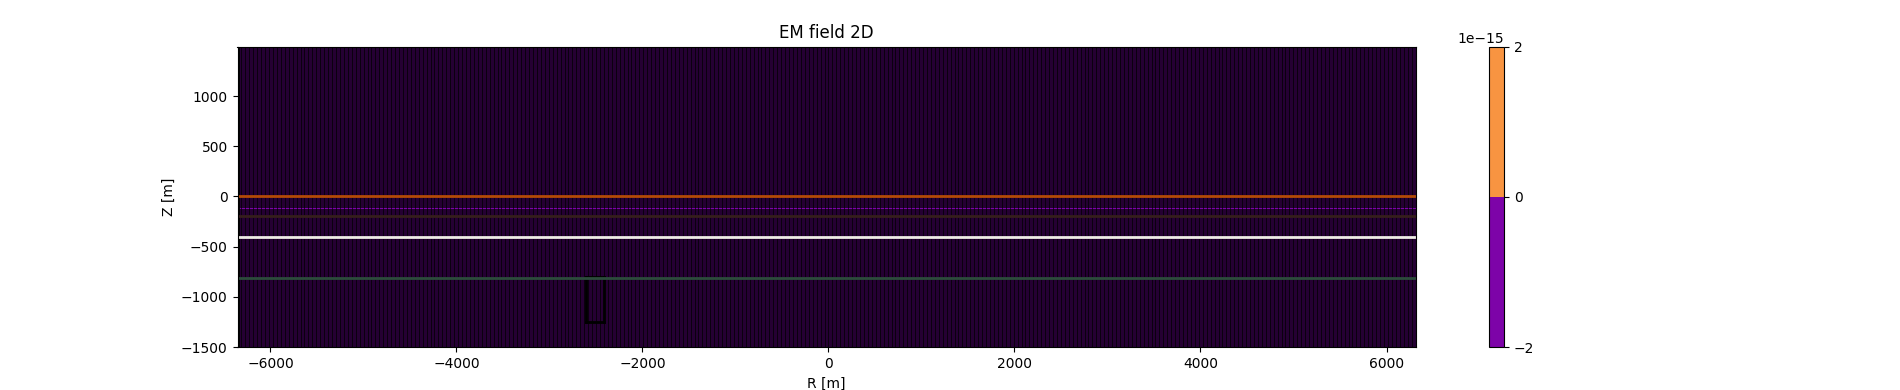
\includegraphics[width=1.0\linewidth]{images/Answer_E_2plus_time_layer_1.png}
	\caption{Решение $\overrightarrow{\textbf{E}}^+$ при $t = 1.0с$}
	\label{fig:E_2plus_t0}
\end{figure} 


\begin{figure}
	\centering
	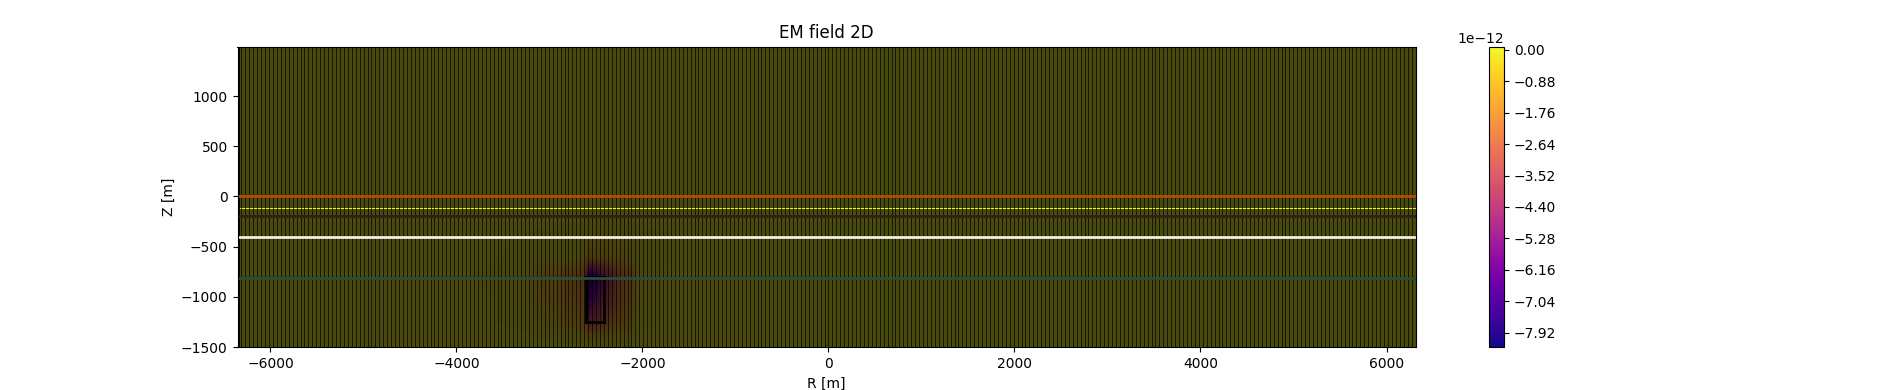
\includegraphics[width=1.0\linewidth]{images/Answer_A_2plus_time_layer_1.0250000000000006.png}
	\caption{Решение $\overrightarrow{\textbf{A}}^+$ при $t = 1.025с$}
	\label{fig:A_2plus_t1}
\end{figure} 


\begin{figure}
	\centering
	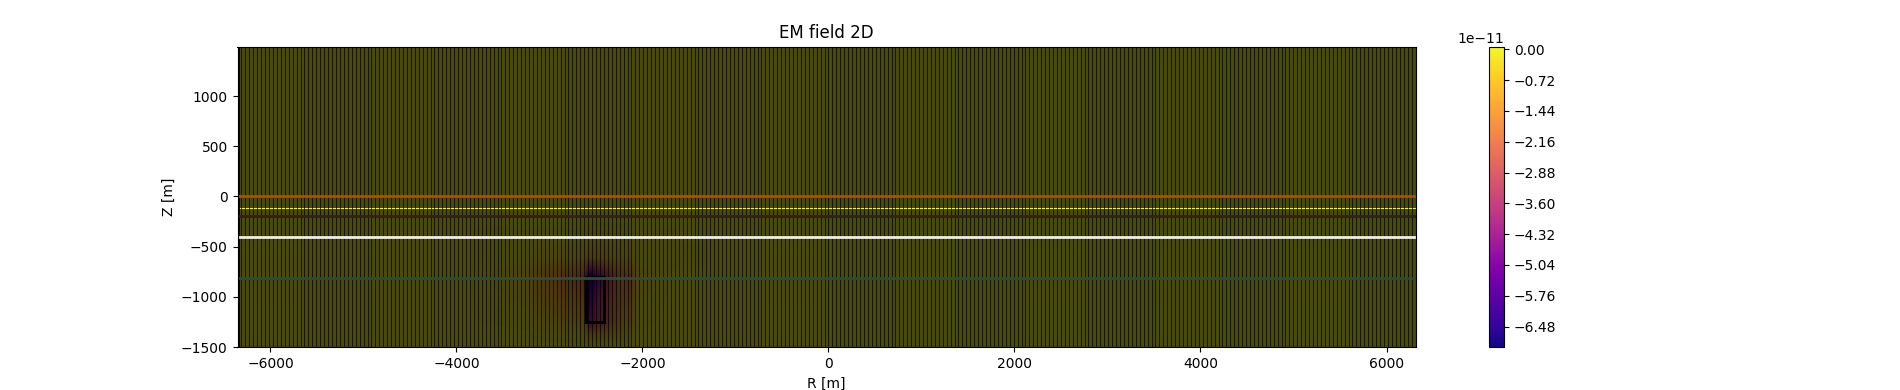
\includegraphics[width=1.0\linewidth]{images/Answer_E_2plus_time_layer_1.0250000000000006.png}
	\caption{Решение $\overrightarrow{\textbf{E}}^+$ при $t = 1.025с$}
	\label{fig:E_2plus_t1}
\end{figure} 

\begin{figure}
	\centering
	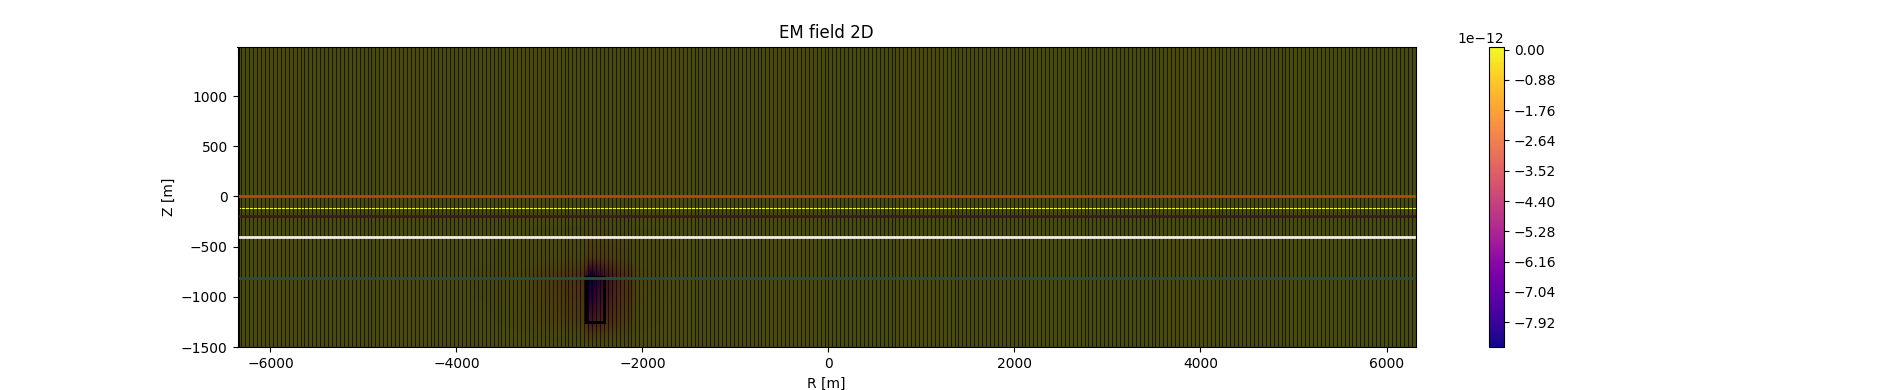
\includegraphics[width=1.0\linewidth]{images/Answer_A_2plus_time_layer_1.05.png}
	\caption{Решение $\overrightarrow{\textbf{A}}^+$ при $t = 1.05с$}
	\label{fig:A_2plus_t2}
\end{figure} 


\begin{figure}
	\centering
	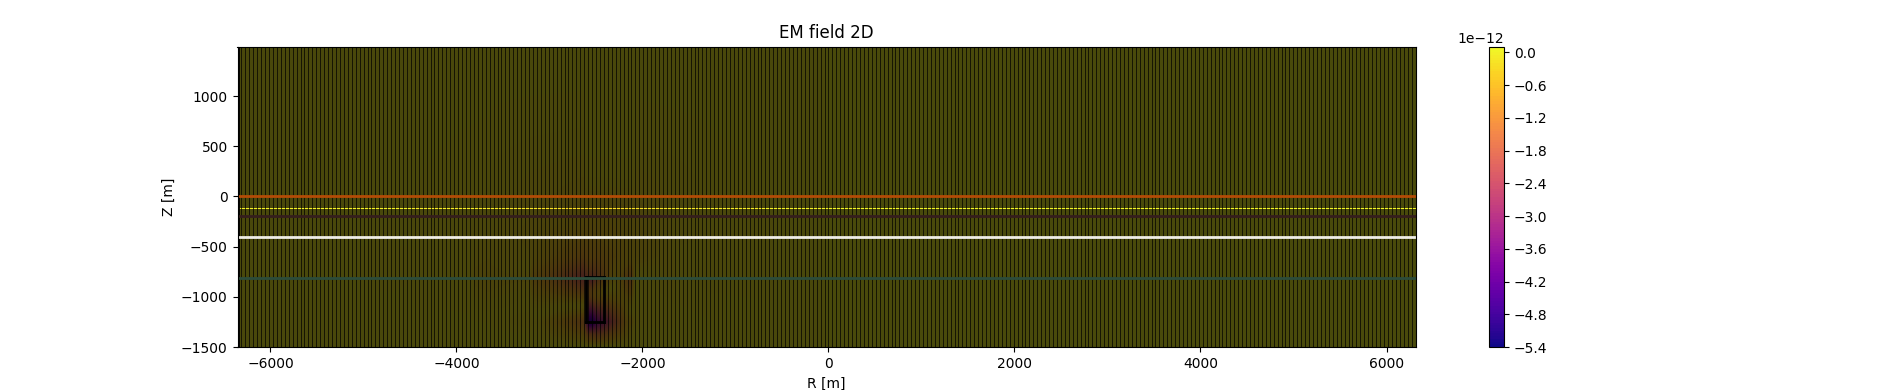
\includegraphics[width=1.0\linewidth]{images/Answer_E_2plus_time_layer_1.05.png}
	\caption{Решение $\overrightarrow{\textbf{E}}^+$ при $t = 1.05с$}
	\label{fig:E_2plus_t2}
\end{figure} 

Рассмотрим для $t = 1.0, t = 1.025, t = 1.05$ значения $\overrightarrow{\textbf{A}}^+$ и $\overrightarrow{\textbf{E}}^+$ на линии, перпендикулярно проходящей к аномальному объекту по оси $y$ при $x = -1177.5, z = -1050.0$. Получим следующее:

\begin{figure}
	\centering
	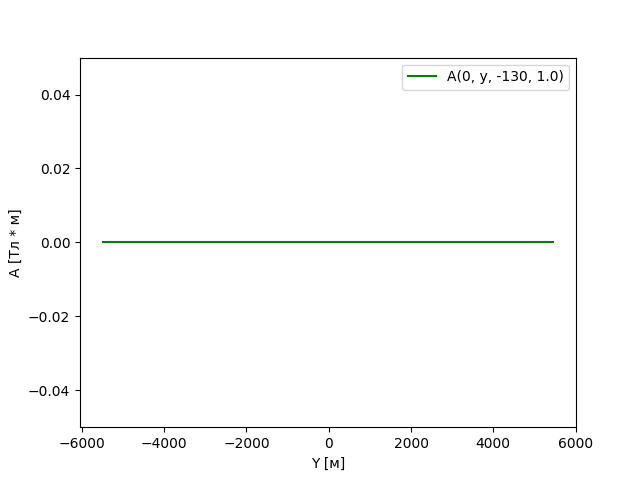
\includegraphics[width=0.5\linewidth]{images/Normal_A_obj2_1.png}
	\caption{Решение $\overrightarrow{\textbf{A}}$ на линии $(0.0, y, -130.0)$ при $t = 1.025с$}
	\label{fig:A_2line_t0}
\end{figure} 

\begin{figure}
	\centering
	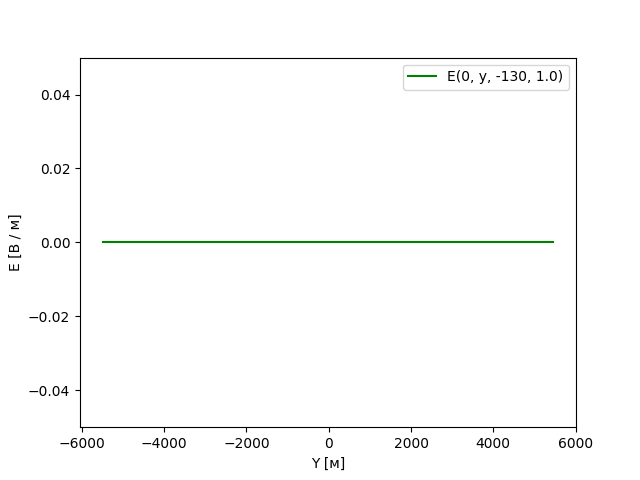
\includegraphics[width=0.5\linewidth]{images/Normal_E_obj2_1.png}
	\caption{Решение $\overrightarrow{\textbf{E}}$ на линии $(0.0, y, -130.0)$ при $t = 1.025с$}
	\label{fig:E_2line_t0}
\end{figure} 

\begin{figure}
	\centering
	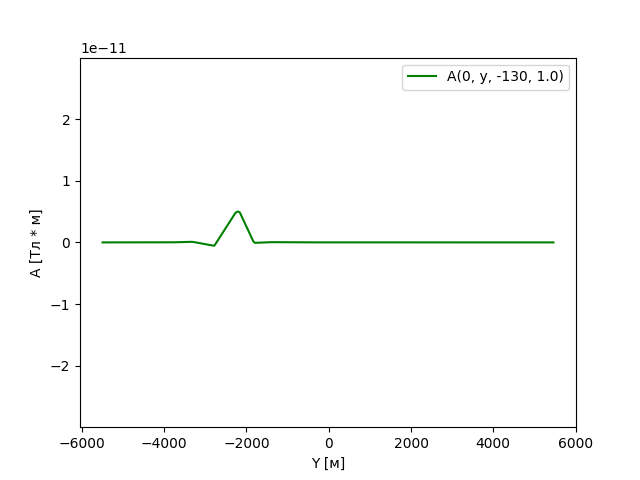
\includegraphics[width=0.5\linewidth]{images/Normal_A_obj2_2.png}
	\caption{Решение $\overrightarrow{\textbf{A}}$ на линии $(0.0, y, -130.0)$ при $t = 1.025с$}
	\label{fig:A_2line_t1}
\end{figure} 

\begin{figure}
	\centering
	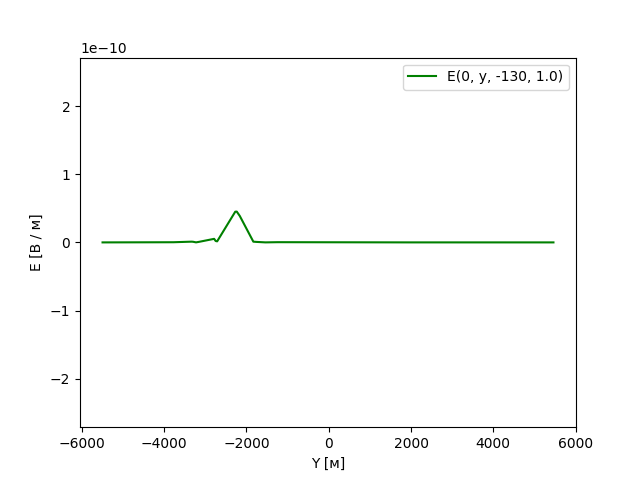
\includegraphics[width=0.5\linewidth]{images/Normal_E_obj2_2.png}
	\caption{Решение $\overrightarrow{\textbf{E}}$ на линии $(0.0, y, -130.0)$  при $t = 1.025с$}
	\label{fig:E_2line_t1}
\end{figure} 

\begin{figure}
	\centering
	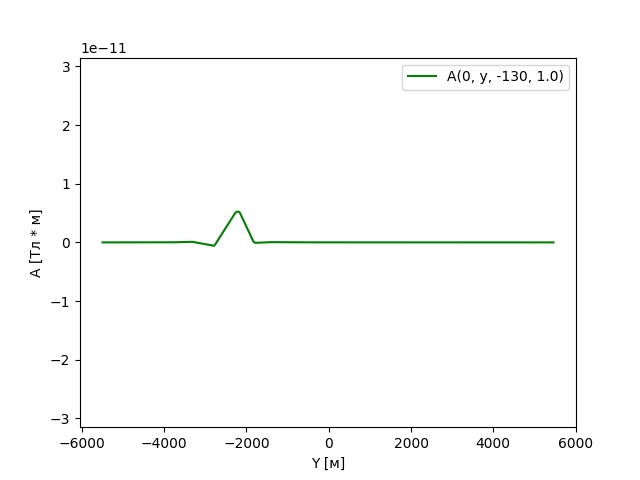
\includegraphics[width=0.5\linewidth]{images/Normal_A_obj2_3.png}
	\caption{Решение $\overrightarrow{\textbf{A}}$ на линии $(0.0, y, -130.0)$  при $t = 1.05с$}
	\label{fig:A_2line_t2}
\end{figure} 

\begin{figure}
	\centering
	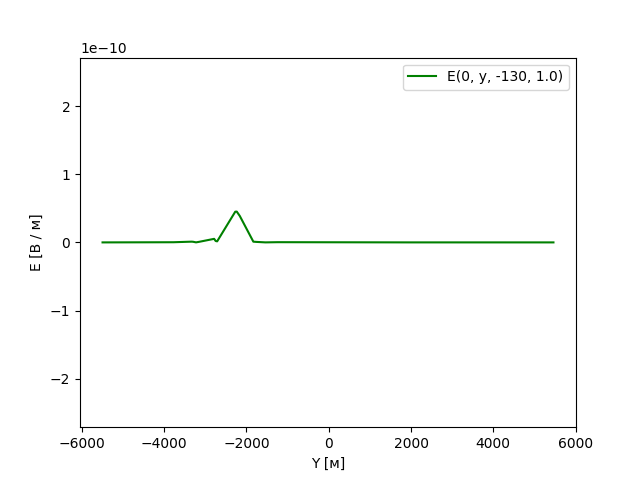
\includegraphics[width=0.5\linewidth]{images/Normal_E_obj2_2.png}
	\caption{Решение $\overrightarrow{\textbf{A}}$ на линии $(0.0, y, -130.0)$  при $t = 1.05с$}
	\label{fig:E_2line_t2}
\end{figure} 

Суммируем полученный результат с полем без аномалий и получим состояние поля в разные моменты времени, изображённые на рисунках \ref{fig:A_IIstage_t0} -- \ref{fig:E_IIstage_t2}.

\begin{figure}
	\centering
	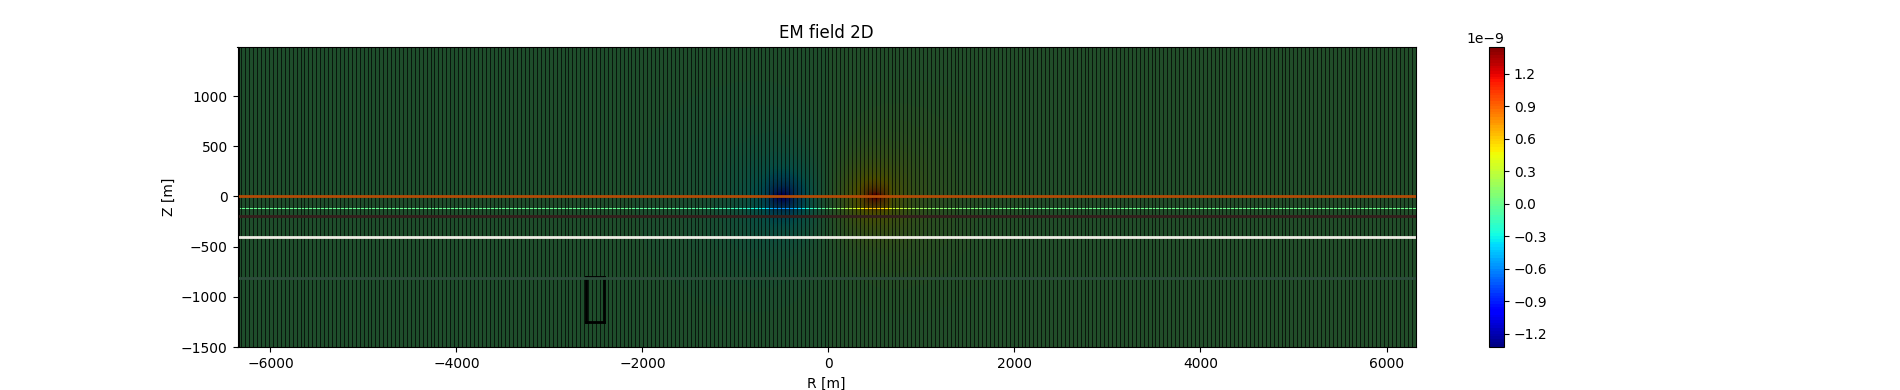
\includegraphics[width=1.0\linewidth]{images/Answer_A_IIstage_time_layer_1.png}
	\caption{Решение суммарного поля $\overrightarrow{\textbf{A}}$ при $t = 1.0с$}
	\label{fig:A_IIstage_t0}
\end{figure} 


\begin{figure}
	\centering
	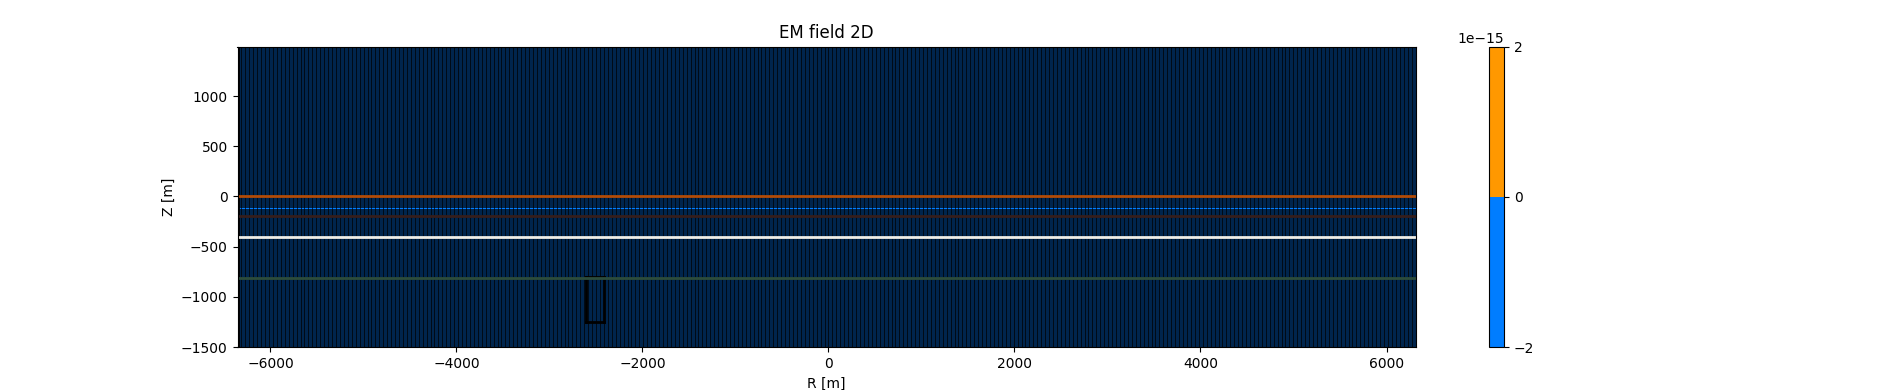
\includegraphics[width=1.0\linewidth]{images/Answer_E_IIstage_time_layer_1.png}
	\caption{Решение суммарного поля $\overrightarrow{\textbf{E}}$ при $t = 1.0с$}
	\label{fig:E_IIstage_t0}
\end{figure} 


\begin{figure}
	\centering
	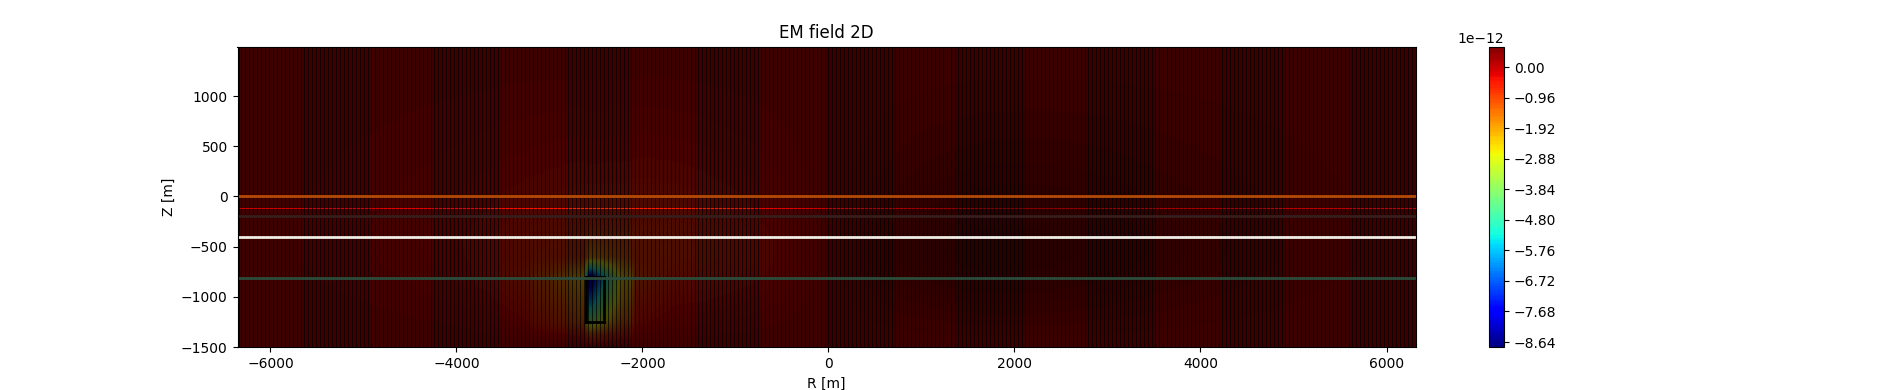
\includegraphics[width=1.0\linewidth]{images/Answer_A_IIstage_time_layer_1.0250000000000006.png}
	\caption{Решение суммарного поля $\overrightarrow{\textbf{A}}$ при $t = 1.025с$}
	\label{fig:A_IIstage_t1}
\end{figure} 


\begin{figure}
	\centering
	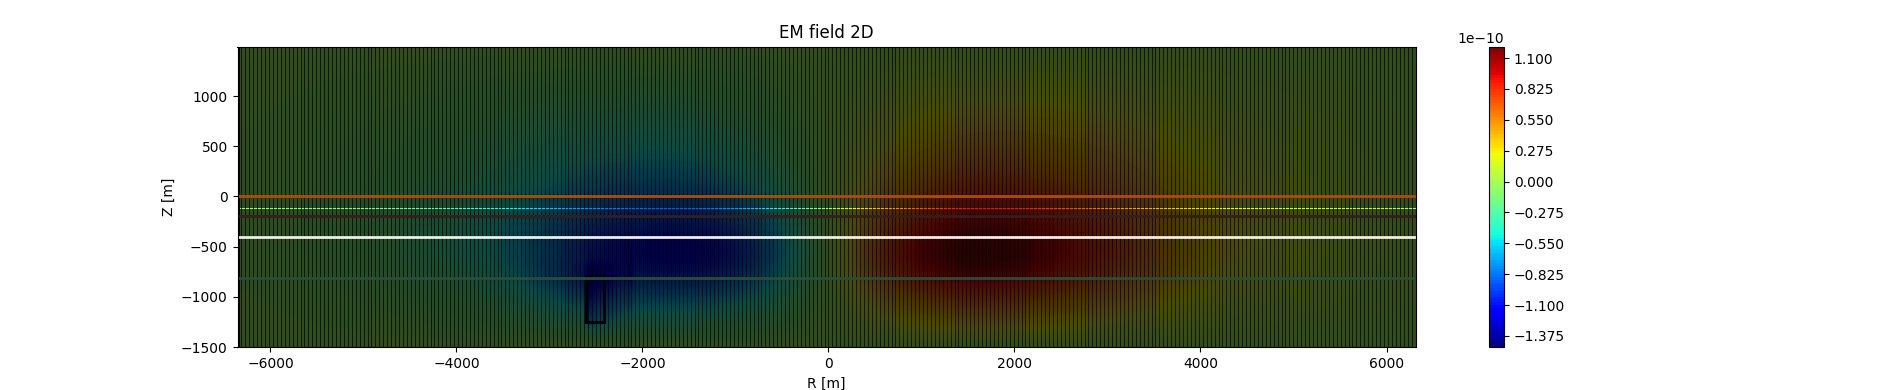
\includegraphics[width=1.0\linewidth]{images/Answer_E_IIstage_time_layer_1.0250000000000006.png}
	\caption{Решение суммарного поля $\overrightarrow{\textbf{E}}$ при $t = 1.025с$}
	\label{fig:E_IIstage_t1}
\end{figure} 

\begin{figure}
	\centering
	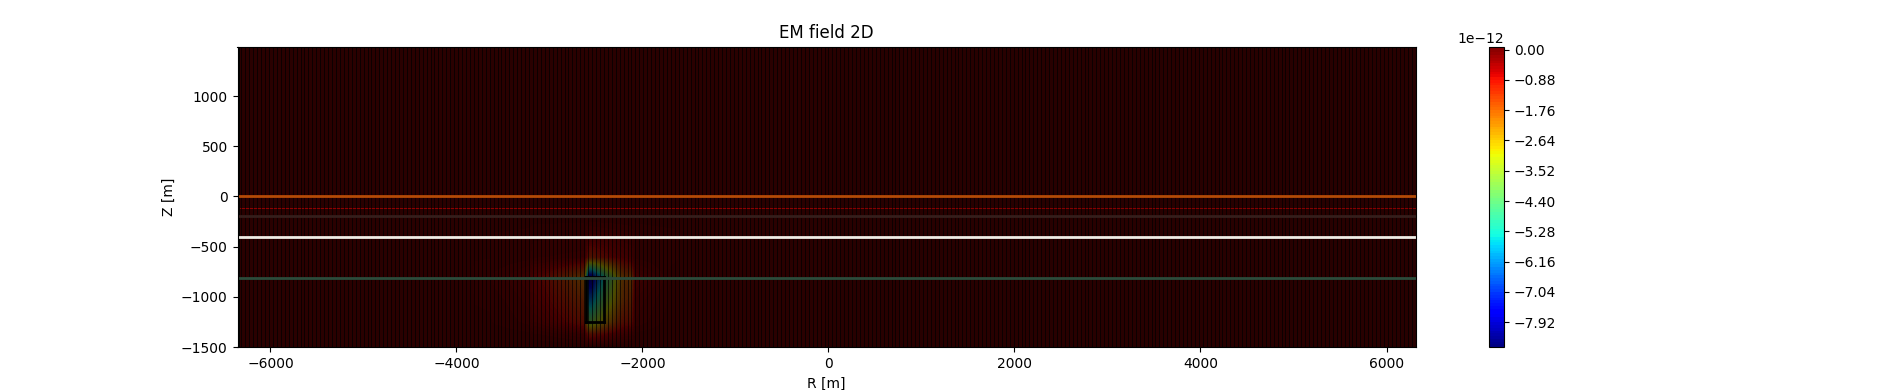
\includegraphics[width=1.0\linewidth]{images/Answer_A_IIstage_time_layer_1.05.png}
	\caption{Решение суммарного поля $\overrightarrow{\textbf{A}}$ при $t = 1.05с$}
	\label{fig:A_IIstage_t2}
\end{figure} 


\begin{figure}
	\centering
	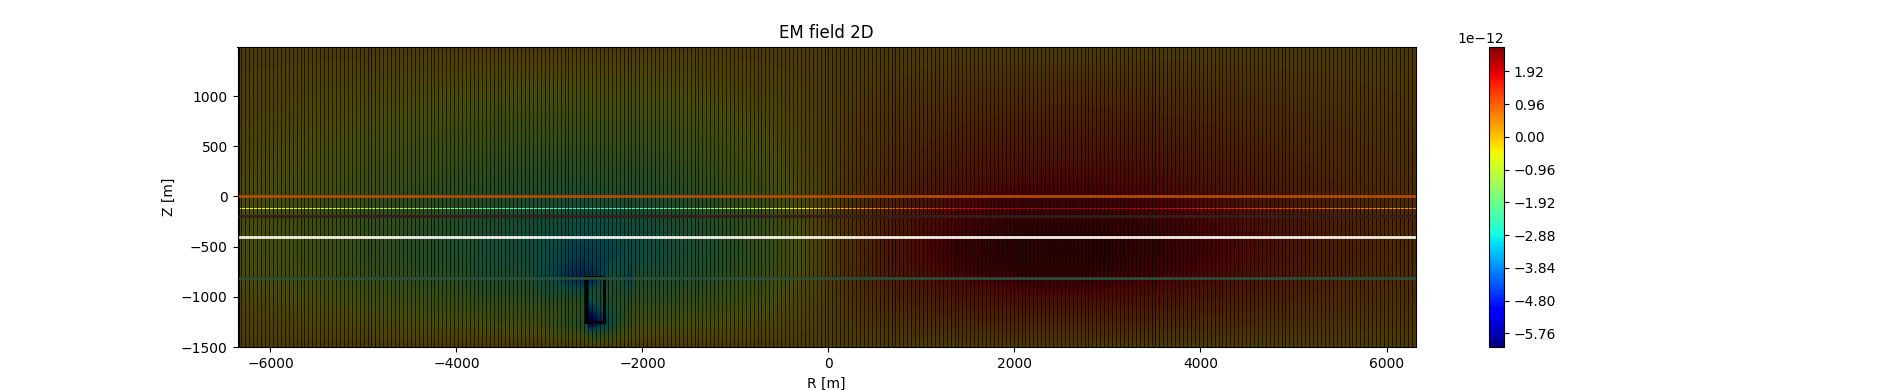
\includegraphics[width=1.0\linewidth]{images/Answer_E_IIstage_time_layer_1.05.png}
	\caption{Решение суммарного поля $\overrightarrow{\textbf{E}}$ при $t = 1.05с$}
	\label{fig:E_IIstage_t2}
\end{figure} 

Полученные значения \ref{fig:A_Log_added2} -- \ref{fig:E_Log_added2} $\overrightarrow{\textbf{A}}$ и $\overrightarrow{\textbf{E}}$ рассмотрим на приёмниках.

\begin{figure}
	\centering
	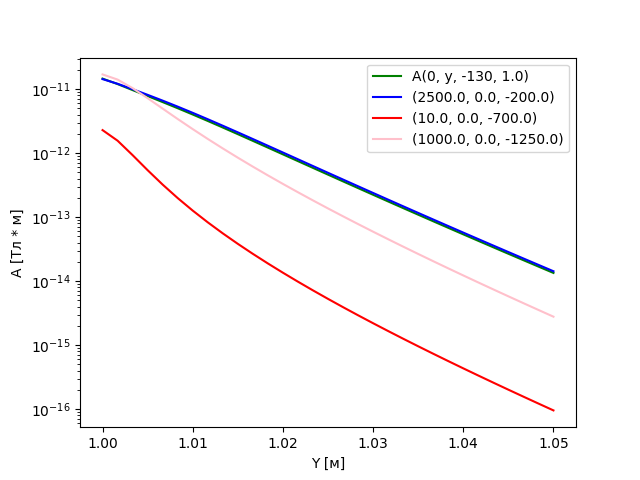
\includegraphics[width=0.8\linewidth]{images/Log_A_obj2.png}
	\caption{Решение суммарного поля $\overrightarrow{\textbf{E}}$ при $t = 1.05с$}
	\label{fig:A_Log_added2}
\end{figure} 


\begin{figure}
	\centering
	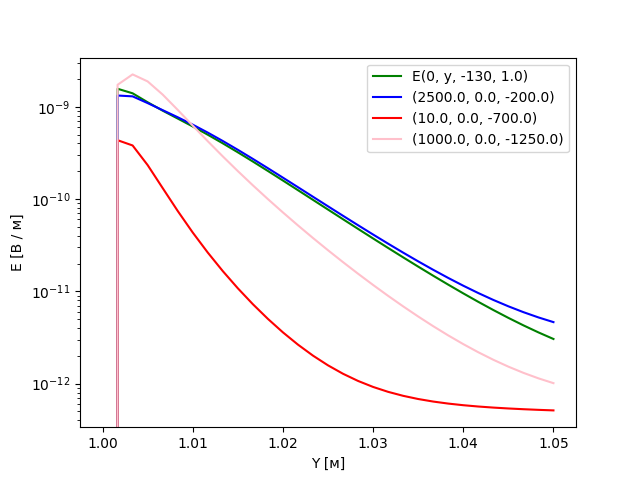
\includegraphics[width=0.8\linewidth]{images/Log_E_obj2.png}
	\caption{Решение суммарного поля $\overrightarrow{\textbf{E}}$ при $t = 1.05с$}
	\label{fig:E_Log_added2}
\end{figure} 

Сравнивая показатели на приёмниках до добавления аномалии \ref{fig:LogA} -- \ref{fig:LogE} и после \ref{fig:A_Log_added2} -- \ref{fig:A_Log_added2}, можно заметить, что значения напряжённости электрического поля ни на одном из приёмников не претерпели изменения, по всей видимости из-за неудачного их расположения. Для изменения ситуации необходимо было бы увеличить размеры расчётной области по пространству и временного диапазона. 

Рассмотрим теперь поле с двумя объектами сразу. Для этого сначала добавим первый объект к чистой расчётной области, после используя его в качестве нормального, добавим вторую аномалию.

\begin{figure}
	\centering
	\includegraphics[width=1.0\linewidth]{images/Answer_A_both_time_layer_1.png}
	\caption{Решение суммарного поля $\overrightarrow{\textbf{A}}$ при $t = 1.0с$}
	\label{fig:A_both_t0}
\end{figure} 


\begin{figure}
	\centering
	\includegraphics[width=1.0\linewidth]{images/Answer_E_both_time_layer_1.png}
	\caption{Решение суммарного поля $\overrightarrow{\textbf{E}}$ при $t = 1.0с$}
	\label{fig:E_both_t0}
\end{figure} 


\begin{figure}
	\centering
	\includegraphics[width=1.0\linewidth]{images/Answer_A_both_time_layer_1.0250000000000006.png}
	\caption{Решение суммарного поля $\overrightarrow{\textbf{A}}$ при $t = 1.025с$}
	\label{fig:A_both_t1}
\end{figure} 


\begin{figure}
	\centering
	\includegraphics[width=1.0\linewidth]{images/Answer_E_both_time_layer_1.0250000000000006.png}
	\caption{Решение суммарного поля $\overrightarrow{\textbf{E}}$ при $t = 1.025с$}
	\label{fig:E_both_t1}
\end{figure} 

\begin{figure}
	\centering
	\includegraphics[width=1.0\linewidth]{images/Answer_A_both_time_layer_1.05.png}
	\caption{Решение суммарного поля $\overrightarrow{\textbf{A}}$ при $t = 1.05с$}
	\label{fig:A_both_t2}
\end{figure} 


\begin{figure}
	\centering
	\includegraphics[width=1.0\linewidth]{images/Answer_E_both_time_layer_1.05.png}
	\caption{Решение суммарного поля $\overrightarrow{\textbf{E}}$ при $t = 1.05с$}
	\label{fig:E_both_t2}
\end{figure} 

Полученные значения \ref{fig:A_Log_both} -- \ref{fig:E_Log_both} $\overrightarrow{\textbf{A}}$ и $\overrightarrow{\textbf{E}}$ рассмотрим на приёмниках.

\begin{figure}
	\centering
	\includegraphics[width=0.8\linewidth]{images/Log_A_both.png}
	\caption{Решение суммарного поля $\overrightarrow{\textbf{E}}$ при $t = 1.05с$}
	\label{fig:A_Log_both}
\end{figure} 


\begin{figure}
	\centering
	\includegraphics[width=0.8\linewidth]{images/Log_E_both.png}
	\caption{Решение суммарного поля $\overrightarrow{\textbf{E}}$ при $t = 1.05с$}
	\label{fig:E_Log_both}
\end{figure} 

Сравнивая показатели на приёмниках до добавления обеих аномалий \ref{fig:LogA} -- \ref{fig:LogE} и после \ref{fig:A_Log_both} -- \ref{fig:E_Log_both}, можно заметить, что значения напряжённости электрического поля на красном приёмнике все те же изменения, что и без учёта второго объекта. Это связано со слабым влиянием второго объекта на приёмники. 
\chapter{Теоретическая часть}

\section{Условие задачи}

Пусть имеется некоторый круглый индукционный источник, с радиусом $R_0$ $<<$ 1000. На рисунке \ref{fig:areaExample} имеем однородные краевые условие на правой и нижней границах, и естественные на левой и верхней границах.

\begin{figure}
	\centering
	\includegraphics[width=0.75\linewidth]{images/"Образец сетки".png}
	\caption{Образец сетки}
	\label{fig:areaExample}
\end{figure}

\section{Математическая постановка}

Будем считать, что электромагнитное поле возбуждается круговым током, а вмещающая среда имеет круговую симметрию. Тогда при условии однородности среды по магнитной проницаемости электромагнитное поле полностью описывается одной компонентой $A_{\varphi} = A_{\varphi}(r, z, t)$ вектор-потенциала $\overline{A}$ (в цилиндрической системе координат), и эта функция $A_{\varphi}(r, z, t)$ может быть найдена из решения двумерного уравнения:

\begin{equation} \label{eq1M}
	-\frac{1}{\mu_0} \Delta A_{\varphi} + \frac{A_{\varphi}}{\mu_0 r^2} + \sigma \frac{\partial A_{\varphi}}{\partial t} = J_{\varphi},
\end{equation}
где: $J_{\varphi}$ - дельта-функция равная 1 в одной из подобластей, описывающей кольцо, и равная 0 в остальных.

Переведем это дифференциальное уравнение в частных производных в слабую форму.

\begin{equation} \label{eq2}
	\int \limits_{\Omega} \left(-\frac{1}{\mu_0} \grad \left(\grad{A_{\varphi}}\right) + \frac{A_{\varphi}}{\mu_0 r^2} + \sigma \frac{\partial A_{\varphi}}{\partial t}\right) v d \Omega = \int \limits_{\Omega} J_{\varphi} v d \Omega.
\end{equation}

\begin{equation} \label{eq3}
	\int \limits_{\Omega} \grad \left( -\frac{1}{\mu_0} \grad{A_{\varphi}}\right) v d \Omega + \int \limits_{\Omega} \frac{A_{\varphi}}{\mu_0 r^2} v d \Omega + \int \limits_{\Omega} \sigma \frac{\partial A_{\varphi}}{\partial t} v d \Omega = \int \limits_{\Omega} J_{\varphi} v d \Omega.
\end{equation}

Применив формулу Гаусса-Остроградского, и принимая во внимание, что по условию задачи в некоторых местах поток через границу равен нулю, получим:

\begin{equation} \label{eq4}
	\int \limits_{\Omega} \frac{1}{\mu_0}   \grad{A_{\varphi}} \grad v d \Omega + \int \limits_{\Omega} \frac{A_{\varphi}}{\mu_0 r^2} v d \Omega + \int \limits_{\Omega} \sigma \frac{\partial A_{\varphi}}{\partial t} v d \Omega - \int \limits_{\Omega} J_{\varphi} v d \Omega = 0.
\end{equation}

\section{Принципы построения локальных векторов, матриц жесткости и масс}
Поскольку решаемое уравнение в $(r, z)$ координатах и имеется особый нелинейный коэффициент $\gamma = \frac{1}{r^2}$, локальные матрицы жесткости и масс для одномерной задачи выглядят следующим образом:

\begin{equation*}
	\hat{G^r} = \hat{\lambda} \frac{r_k + h_k / 2}{h_k} \left(
	\begin{array}{rr}
		 1 & -1\\
		-1 &  1\\
	\end{array}
	\right),
\end{equation*}

\begin{equation*}
    \hat{M^r} = \ln\left(1 + \frac{1}{d}\right)
	\left(
	\begin{array}{cc}
		(1+d)^2 & -d(1+d)\\
		-d(1+d) &  d^2\\
	\end{array}
	\right)
	-d
	\left(
	\begin{array}{rr}
		1 & -1\\
		-1 & 1\\
	\end{array}
	\right)
	+ \frac{1}{2}
	\left(
	\begin{array}{rr}
		-3 & 1\\
		1 & 1\\
	\end{array}
	\right)
\end{equation*}
где $d = \frac{r_k}{h_k}$.


\begin{equation*}
	\hat{G^z} = \frac{\hat{\lambda}}{h_k} \left(
	\begin{array}{rr}
		1 & -1\\
		-1 &  1\\
	\end{array}
	\right),
\end{equation*}

\begin{equation*}
	\hat{M^z} = \frac{\hat{\gamma} h_k}{6} \left(
	\begin{array}{rr}
		2 & 1\\
		1 & 2\\
	\end{array}
	\right).
\end{equation*}

Тогда элементы верхнего треугольника матрицы жесткости для двумерных задач, можем представить в виде:

\begin{equation*}
	\begin{array}{ll}
		\hat{G}_{11} = \hat{\lambda}\left(G^r_{11}M^z_{11} + M^r_{11}G^z_{11}\right), & \hat{G}_{12} = \hat{\lambda}\left(G^r_{12}M^z_{11} + M^r_{12}G^z_{11}\right),\\
		\hat{G}_{13} = \hat{\lambda}\left(G^r_{11}M^z_{12} + M^r_{11}G^z_{12}\right), & \hat{G}_{14} = \hat{\lambda}\left(G^r_{12}M^z_{12} + M^r_{12}G^z_{12}\right),\\
		\hat{G}_{22} = \hat{\lambda}\left(G^r_{22}M^z_{11} + M^r_{22}G^z_{11}\right), & \hat{G}_{23} = \hat{\lambda}\left(G^r_{21}M^z_{12} + M^r_{21}G^z_{12}\right),\\
		\hat{G}_{24} = \hat{\lambda}\left(G^r_{22}M^z_{12} + M^r_{22}G^z_{12}\right), & \hat{G}_{33} = \hat{\lambda}\left(G^r_{11}M^z_{22} + M^r_{11}G^z_{22}\right),\\
		\hat{G}_{34} = \hat{\lambda}\left(G^r_{12}M^z_{22} + M^r_{12}G^z_{22}\right), & \hat{G}_{44} = \hat{\lambda}\left(G^r_{22}M^z_{22} + M^r_{22}G^z_{22}\right).\\
	\end{array}
\end{equation*}

Верхний треугольник элементов матрицы масс может быть представлены в виде:

\begin{equation*}
	\begin{array}{ll}
		\hat{M}_{11} = \hat{\gamma}M^r_{11}M^z_{11}, & \hat{M}_{12} = \hat{\gamma}M^r_{12}M^z_{11},\\
		\hat{M}_{13} = \hat{\gamma}M^r_{11}M^z_{12}, & \hat{M}_{14} = \hat{\gamma}M^r_{12}M^z_{12},\\
		\hat{M}_{22} = \hat{\gamma}M^r_{22}M^z_{11}, & \hat{M}_{23} = \hat{\gamma}M^r_{21}M^z_{12},\\
		\hat{M}_{24} = \hat{\gamma}M^r_{22}M^z_{12}, & \hat{M}_{33} = \hat{\gamma}M^r_{11}M^z_{22},\\
		\hat{M}_{34} = \hat{\gamma}M^r_{12}M^z_{22}, & \hat{M}_{44} = \hat{\gamma}M^r_{22}M^z_{22}.\\
	\end{array}
\end{equation*}

Выразим матрицу $\hat{M}$ следующим образом:

\begin{equation*}
	\hat{M} = \hat{\gamma} \hat{C}.
\end{equation*}

Для генерации вектора правой части, воспользуемся следующим соотношением:

\begin{equation*}
	\hat{b} = \hat{C} \hat{f}.
\end{equation*}
 
 
\section{Аппроксимация краевой задачи по времени}

Представим искомое решение $u$ на интервале $\left(t_{j-2}, t_j\right)$ в следующем виде:

\begin{equation} \label{eq5m}
	u(r, z, t) \approx u^{j-2}(r, z)\eta_2^j(t) + u^{j-1}(r, z)\eta_1^j(t) + u^{j}(r, z)\eta_0^j(t).
\end{equation}

где функции $\eta_2^j(t)$, $\eta_1^j(t)$, $\eta_0^j(t)$ - базисные квадратичные полиномы Лагранжа (с двумя корнями из набора значений времен $t_{j-2}$, $t_{j-1}$, $t_j$), которые могут быть записаны в виде:

\begin{equation*}
	\eta_2^j(t) = \frac{1}{\Delta t_1 \Delta t} \left(t - t_{j-1}\right) \left(t-t_j\right),
\end{equation*}

\begin{equation*}
	\eta_1^j(t) = -\frac{1}{\Delta t_1 \Delta t_0} \left(t - t_{j-2}\right) \left(t-t_j\right),
\end{equation*}

\begin{equation*}
	\eta_0^j(t) = \frac{1}{\Delta t \Delta t_0} \left(t - t_{j-2}\right) \left(t-t_{j-1}\right),
\end{equation*}
где:

\begin{equation*}
	\begin{array}{ccc}
	\Delta t = t_j - t_{j - 2},&
	\Delta t_1 = t_{j - 1} - t_{j - 2},&
	\Delta t_0 = t_j - t_{j - 1}.
	\end{array}
\end{equation*}


Применим представление \ref{eq5m} для аппроксимации производной по времени параболического уравнения \ref{eq1M} на временном слое $t = t_j$:

\begin{equation} \label{cabel}
	\sigma \frac{\partial}{\partial t} \left(u^{j-2}(r, z) \eta_2^j(t) + u^{j-1}(r, z) \eta_1^j(t) + u^j(r, z) \eta_0^j(t)\right) -\frac{1}{\mu_0} \Delta A_{\varphi} + \frac{A_{\varphi}}{\mu_0 r^2} = J_{\varphi}
\end{equation}

Выполняя конечноэлементную аппроксимацию краевой задачи для уравнения \ref{cabel}, получим СЛАУ следующего вида:


\begin{multline} \label{gabel}
	\left(\frac{\Delta t + \Delta t_0}{\Delta t \Delta t_0} M + G + M\right)q^{j} = b^{j} - \frac{\Delta t_0}{\Delta t \Delta t_1} M q^{j - 2} + \frac{\Delta t}{\Delta t_1 \Delta t_0} M q^{j - 1}.
\end{multline}

% Далее глава тестирования.
\chapter{Исследования}

\section{Исследование первичного поля}

Пусть источник индукционного поля лежит на расстоянии $R = 500$ м от оси симметрии и имееет силу тока, равную $J_{\varphi} = 1.0$ А. Также условимся, что источник работал достаточно долго, чтобы создать стабильное электромагнитное поле. Сетка по времени равномерная: $t=[1.0; 1.05]$ на 200 временных слоёв. После истечения первой секунды мы отключим наш источник, т.е. $J_{\varphi} = 0.0$ A при $t > 1.0$. На рисунках \ref{fig:A_phi_0} -- \ref{fig:E_phi_2} представлено распространение этого поля в среде в начальный, промежуточных и последний момент времени.

\begin{figure}
	\centering
	\includegraphics[width=1.0\linewidth]{images/Answer_A_time_layer_1.png}
	\caption{Решение $A_{\varphi}$ при $t = 1.0с$}
	\label{fig:A_phi_0}
\end{figure}

\begin{figure}
	\centering
	\includegraphics[width=1.0\linewidth]{images/Answer_E_time_layer_1.png}
	\caption{Решение $E_{\varphi}$ при $t = 1.0с$}
	\label{fig:E_phi_0}
\end{figure}

\begin{figure}
	\centering
	\includegraphics[width=1.0\linewidth]{images/Answer_A_time_layer_1.0250000000000083.png}
	\caption{Решение $A_{\varphi}$ при $t = 1.025с$}
	\label{fig:A_phi_1}
\end{figure}

\begin{figure}
	\centering
	\includegraphics[width=1.0\linewidth]{images/Answer_E_time_layer_1.0250000000000083.png}
	\caption{Решение $E_{\varphi}$ при $t = 1.025с$}
	\label{fig:E_phi_1}
\end{figure} 

\begin{figure}
	\centering
	\includegraphics[width=1.0\linewidth]{images/Answer_A_time_layer_1.05.png}
	\caption{Решение $A_{\varphi}$ при $t = 1.05с$}
	\label{fig:A_phi_2}
\end{figure}

\begin{figure}
	\centering
	\includegraphics[width=1.0\linewidth]{images/Answer_E_time_layer_1.05.png}
	\caption{Решение $A_{\varphi}$ при $t = 1.05с$}
	\label{fig:E_phi_2}
\end{figure} 

Расположим на расчётной области приёмники в каждой горизонтально-слоистой среде и проведем замеры значений вектор-потенциала и электрического поля в точках $(2500; 0; -100)$, $(2500; 0; -200)$, $(10; 0; -700)$, $(1000; 0; -1250)$. Отобразим на графиках \ref{fig:NatA} -- \ref{fig:LogE} полученные значения.

\begin{figure}
	\centering
	\includegraphics[width=0.8\linewidth]{images/Normal_A.png}
	\caption{Зависимость значения $A_{\varphi}$ от времени в разных приёмниках}
	\label{fig:NatA}
\end{figure}

\begin{figure}
	\centering
	\includegraphics[width=0.8\linewidth]{images/Normal_E.png}
	\caption{Зависимость значения $E_{\varphi}$ от времени в разных приёмниках}
	\label{fig:NatE}
\end{figure}


\begin{figure}
	\centering
	\includegraphics[width=0.8\linewidth]{images/Log_A.png}
	\caption{Зависимость значения $A_{\varphi}$ от времени в разных приёмниках (логарифмическая шкала по оси абсцисс)}
	\label{fig:LogA}
\end{figure}

\begin{figure}
	\centering
	\includegraphics[width=0.8\linewidth]{images/Log_E.png}
	\caption{Зависимость значения $E_{\varphi}$ от времени в разных приёмниках (логарифмическая шкала по оси абсцисс)}
	\label{fig:LogE}
\end{figure} 

Как видим, значения вектор-потенциала и электрической напряжённости поля не имеют каких-либо резких колебаний. Из этого можно заключить, что, как и предполагалось, никаких аномальных зон в исследуемой области нет. 

\section{Исследование при разделении нормального и добавочного поля}

Добавим в нашу область аномальный объект со следующими границами: $[-5500; 5500]_x \times [2205; 2355]_y \times [-180; -80]_z$ и значением $\sigma = 4$. Будем искать решение из уравнения на добавочное поле (\ref{eq_1_6}). Получим решения изображенные на рисунках \ref{fig:A_plus_t0} -- \ref{fig:E_plus_t2}.

\begin{figure}
	\centering
	\includegraphics[width=1.0\linewidth]{images/Answer_A_plus_time_layer_1.png}
	\caption{Решение $\overrightarrow{\textbf{A}}^+$ при $t = 1.0с$}
	\label{fig:A_plus_t0}
\end{figure} 


\begin{figure}
	\centering
	\includegraphics[width=1.0\linewidth]{images/Answer_E_plus_time_layer_1.png}
	\caption{Решение $\overrightarrow{\textbf{E}}^+$ при $t = 1.0с$}
	\label{fig:E_plus_t0}
\end{figure} 


\begin{figure}
	\centering
	\includegraphics[width=1.0\linewidth]{images/Answer_A_plus_time_layer_1.0250000000000006.png}
	\caption{Решение $\overrightarrow{\textbf{A}}^+$ при $t = 1.025с$}
	\label{fig:A_plus_t1}
\end{figure} 


\begin{figure}
	\centering
	\includegraphics[width=1.0\linewidth]{images/Answer_E_plus_time_layer_1.0250000000000006.png}
	\caption{Решение $\overrightarrow{\textbf{E}}^+$ при $t = 1.025с$}
	\label{fig:E_plus_t1}
\end{figure} 

\begin{figure}
	\centering
	\includegraphics[width=1.0\linewidth]{images/Answer_A_plus_time_layer_1.05.png}
	\caption{Решение $\overrightarrow{\textbf{A}}^+$ при $t = 1.05с$}
	\label{fig:A_plus_t2}
\end{figure} 


\begin{figure}
	\centering
	\includegraphics[width=1.0\linewidth]{images/Answer_E_plus_time_layer_1.05.png}
	\caption{Решение $\overrightarrow{\textbf{E}}^+$ при $t = 1.05с$}
	\label{fig:E_plus_t2}
\end{figure} 

Рассмотрим для $t = 1.0, t = 1.025, t = 1.05$ значения $\overrightarrow{\textbf{A}}^+$ и $\overrightarrow{\textbf{E}}^+$ на линии, перпендикулярно проходящей к аномальному объекту по оси $y$ при $x = 0.0, z = -130.0$. Получим следующее:

\begin{figure}
	\centering
	\includegraphics[width=0.5\linewidth]{images/Normal_A(y)_1.png}
	\caption{Решение $\overrightarrow{\textbf{A}}^+$ на линии $(0.0, y, -130.0)$ при $t = 1.0с$}
	\label{fig:A_line_t0}
\end{figure} 

\begin{figure}
	\centering
	\includegraphics[width=0.5\linewidth]{images/Normal_E(y)_1.png}
	\caption{Решение $\overrightarrow{\textbf{E}}^+$ на линии $(0.0, y, -130.0)$ при $t = 1.0с$}
	\label{fig:E_line_t0}
\end{figure} 

\begin{figure}
	\centering
	\includegraphics[width=0.5\linewidth]{images/Normal_A(y)_2.png}
	\caption{Решение $\overrightarrow{\textbf{A}}^+$ на линии $(0.0, y, -130.0)$ при $t = 1.025с$}
	\label{fig:A_line_t1}
\end{figure} 

\begin{figure}
	\centering
	\includegraphics[width=0.5\linewidth]{images/Normal_E(y)_2.png}
	\caption{Решение $\overrightarrow{\textbf{E}}^+$ на линии $(0.0, y, -130.0)$  при $t = 1.025с$}
	\label{fig:E_line_t1}
\end{figure} 

\begin{figure}
	\centering
	\includegraphics[width=0.5\linewidth]{images/Normal_A(y)_3.png}
	\caption{Решение $\overrightarrow{\textbf{A}}^+$ на линии $(0.0, y, -130.0)$  при $t = 1.05с$}
	\label{fig:A_line_t2}
\end{figure} 

\begin{figure}
	\centering
	\includegraphics[width=0.5\linewidth]{images/Normal_A(y)_3.png}
	\caption{Решение $\overrightarrow{\textbf{A}}^+$ на линии $(0.0, y, -130.0)$  при $t = 1.05с$}
	\label{fig:E_line_t2}
\end{figure} 


Суммируем полученный результат с нормальным полем и получим состояние поля в разные моменты времени, изображённые на рисунках \ref{fig:A_Istage_t0} -- \ref{fig:E_Istage_t2}.

\begin{figure}
	\centering
	\includegraphics[width=1.0\linewidth]{images/Answer_A_Istage_time_layer_1.png}
	\caption{Решение суммарного поля $\overrightarrow{\textbf{A}}$ при $t = 1.0с$}
	\label{fig:A_Istage_t0}
\end{figure} 


\begin{figure}
	\centering
	\includegraphics[width=1.0\linewidth]{images/Answer_E_Istage_time_layer_1.png}
	\caption{Решение суммарного поля $\overrightarrow{\textbf{E}}$ при $t = 1.0с$}
	\label{fig:E_Istage_t0}
\end{figure} 


\begin{figure}
	\centering
	\includegraphics[width=1.0\linewidth]{images/Answer_A_Istage_time_layer_1.0250000000000006.png}
	\caption{Решение суммарного поля $\overrightarrow{\textbf{A}}$ при $t = 1.025с$}
	\label{fig:A_Istage_t1}
\end{figure} 


\begin{figure}
	\centering
	\includegraphics[width=1.0\linewidth]{images/Answer_E_Istage_time_layer_1.0250000000000006.png}
	\caption{Решение суммарного поля $\overrightarrow{\textbf{E}}$ при $t = 1.025с$}
	\label{fig:E_Istage_t1}
\end{figure} 

\begin{figure}
	\centering
	\includegraphics[width=1.0\linewidth]{images/Answer_A_Istage_time_layer_1.05.png}
	\caption{Решение суммарного поля $\overrightarrow{\textbf{A}}$ при $t = 1.05с$}
	\label{fig:A_Istage_t2}
\end{figure} 


\begin{figure}
	\centering
	\includegraphics[width=1.0\linewidth]{images/Answer_E_Istage_time_layer_1.05.png}
	\caption{Решение суммарного поля $\overrightarrow{\textbf{E}}$ при $t = 1.05с$}
	\label{fig:E_Istage_t2}
\end{figure} 

Полученные значения \ref{fig:A_Log_added} -- \ref{fig:E_Log_added} $\overrightarrow{\textbf{A}}$ и $\overrightarrow{\textbf{E}}$ рассмотрим на приёмниках.

\begin{figure}
	\centering
	\includegraphics[width=0.8\linewidth]{images/Log_A_obj1.png}
	\caption{Решение суммарного поля $\overrightarrow{\textbf{E}}$ при $t = 1.05с$}
	\label{fig:A_Log_added}
\end{figure} 


\begin{figure}
	\centering
	\includegraphics[width=0.8\linewidth]{images/Log_E_obj1.png}
	\caption{Решение суммарного поля $\overrightarrow{\textbf{E}}$ при $t = 1.05с$}
	\label{fig:E_Log_added}
\end{figure} 

Сравнивая показатели на приёмниках до добавления аномалии \ref{fig:LogA} -- \ref{fig:LogE} и после \ref{fig:A_Log_added} -- \ref{fig:A_Log_added}, можно заметить, что значения напряжённости электрического поля на красном приёмнике претерпели наиболее сильные изменения, т.к. он стал более похожим на гиперболу, нежели прямую линию. Значения на синем приёмнике начали изменяться уже в последние сотые секунды исследования. 

\section{Исследование многоэтапного разделения нормального и добавочных полей}

Добавим ещё один аномальный объект со следующими границами: $[-1305; -1050]_x \times [-2255; -2178]_y \times [-1250; -800]_z$ и значением $\sigma = 17$. Будем искать решение из уравнения на добавочное поле (\ref{eq_1_6}). Получим решения в разные моменты времени изображенные на рисунках \ref{fig:A_2plus_t0} -- \ref{fig:E_2plus_t2}.

\begin{figure}
	\centering
	\includegraphics[width=1.0\linewidth]{images/Answer_A_2plus_time_layer_1.png}
	\caption{Решение $\overrightarrow{\textbf{A}}^+$ при $t = 1.0с$}
	\label{fig:A_2plus_t0}
\end{figure} 


\begin{figure}
	\centering
	\includegraphics[width=1.0\linewidth]{images/Answer_E_2plus_time_layer_1.png}
	\caption{Решение $\overrightarrow{\textbf{E}}^+$ при $t = 1.0с$}
	\label{fig:E_2plus_t0}
\end{figure} 


\begin{figure}
	\centering
	\includegraphics[width=1.0\linewidth]{images/Answer_A_2plus_time_layer_1.0250000000000006.png}
	\caption{Решение $\overrightarrow{\textbf{A}}^+$ при $t = 1.025с$}
	\label{fig:A_2plus_t1}
\end{figure} 


\begin{figure}
	\centering
	\includegraphics[width=1.0\linewidth]{images/Answer_E_2plus_time_layer_1.0250000000000006.png}
	\caption{Решение $\overrightarrow{\textbf{E}}^+$ при $t = 1.025с$}
	\label{fig:E_2plus_t1}
\end{figure} 

\begin{figure}
	\centering
	\includegraphics[width=1.0\linewidth]{images/Answer_A_2plus_time_layer_1.05.png}
	\caption{Решение $\overrightarrow{\textbf{A}}^+$ при $t = 1.05с$}
	\label{fig:A_2plus_t2}
\end{figure} 


\begin{figure}
	\centering
	\includegraphics[width=1.0\linewidth]{images/Answer_E_2plus_time_layer_1.05.png}
	\caption{Решение $\overrightarrow{\textbf{E}}^+$ при $t = 1.05с$}
	\label{fig:E_2plus_t2}
\end{figure} 

Рассмотрим для $t = 1.0, t = 1.025, t = 1.05$ значения $\overrightarrow{\textbf{A}}^+$ и $\overrightarrow{\textbf{E}}^+$ на линии, перпендикулярно проходящей к аномальному объекту по оси $y$ при $x = -1177.5, z = -1050.0$. Получим следующее:

\begin{figure}
	\centering
	\includegraphics[width=0.5\linewidth]{images/Normal_A_obj2_1.png}
	\caption{Решение $\overrightarrow{\textbf{A}}$ на линии $(0.0, y, -130.0)$ при $t = 1.025с$}
	\label{fig:A_2line_t0}
\end{figure} 

\begin{figure}
	\centering
	\includegraphics[width=0.5\linewidth]{images/Normal_E_obj2_1.png}
	\caption{Решение $\overrightarrow{\textbf{E}}$ на линии $(0.0, y, -130.0)$ при $t = 1.025с$}
	\label{fig:E_2line_t0}
\end{figure} 

\begin{figure}
	\centering
	\includegraphics[width=0.5\linewidth]{images/Normal_A_obj2_2.png}
	\caption{Решение $\overrightarrow{\textbf{A}}$ на линии $(0.0, y, -130.0)$ при $t = 1.025с$}
	\label{fig:A_2line_t1}
\end{figure} 

\begin{figure}
	\centering
	\includegraphics[width=0.5\linewidth]{images/Normal_E_obj2_2.png}
	\caption{Решение $\overrightarrow{\textbf{E}}$ на линии $(0.0, y, -130.0)$  при $t = 1.025с$}
	\label{fig:E_2line_t1}
\end{figure} 

\begin{figure}
	\centering
	\includegraphics[width=0.5\linewidth]{images/Normal_A_obj2_3.png}
	\caption{Решение $\overrightarrow{\textbf{A}}$ на линии $(0.0, y, -130.0)$  при $t = 1.05с$}
	\label{fig:A_2line_t2}
\end{figure} 

\begin{figure}
	\centering
	\includegraphics[width=0.5\linewidth]{images/Normal_E_obj2_2.png}
	\caption{Решение $\overrightarrow{\textbf{A}}$ на линии $(0.0, y, -130.0)$  при $t = 1.05с$}
	\label{fig:E_2line_t2}
\end{figure} 

Суммируем полученный результат с полем без аномалий и получим состояние поля в разные моменты времени, изображённые на рисунках \ref{fig:A_IIstage_t0} -- \ref{fig:E_IIstage_t2}.

\begin{figure}
	\centering
	\includegraphics[width=1.0\linewidth]{images/Answer_A_IIstage_time_layer_1.png}
	\caption{Решение суммарного поля $\overrightarrow{\textbf{A}}$ при $t = 1.0с$}
	\label{fig:A_IIstage_t0}
\end{figure} 


\begin{figure}
	\centering
	\includegraphics[width=1.0\linewidth]{images/Answer_E_IIstage_time_layer_1.png}
	\caption{Решение суммарного поля $\overrightarrow{\textbf{E}}$ при $t = 1.0с$}
	\label{fig:E_IIstage_t0}
\end{figure} 


\begin{figure}
	\centering
	\includegraphics[width=1.0\linewidth]{images/Answer_A_IIstage_time_layer_1.0250000000000006.png}
	\caption{Решение суммарного поля $\overrightarrow{\textbf{A}}$ при $t = 1.025с$}
	\label{fig:A_IIstage_t1}
\end{figure} 


\begin{figure}
	\centering
	\includegraphics[width=1.0\linewidth]{images/Answer_E_IIstage_time_layer_1.0250000000000006.png}
	\caption{Решение суммарного поля $\overrightarrow{\textbf{E}}$ при $t = 1.025с$}
	\label{fig:E_IIstage_t1}
\end{figure} 

\begin{figure}
	\centering
	\includegraphics[width=1.0\linewidth]{images/Answer_A_IIstage_time_layer_1.05.png}
	\caption{Решение суммарного поля $\overrightarrow{\textbf{A}}$ при $t = 1.05с$}
	\label{fig:A_IIstage_t2}
\end{figure} 


\begin{figure}
	\centering
	\includegraphics[width=1.0\linewidth]{images/Answer_E_IIstage_time_layer_1.05.png}
	\caption{Решение суммарного поля $\overrightarrow{\textbf{E}}$ при $t = 1.05с$}
	\label{fig:E_IIstage_t2}
\end{figure} 

Полученные значения \ref{fig:A_Log_added2} -- \ref{fig:E_Log_added2} $\overrightarrow{\textbf{A}}$ и $\overrightarrow{\textbf{E}}$ рассмотрим на приёмниках.

\begin{figure}
	\centering
	\includegraphics[width=0.8\linewidth]{images/Log_A_obj2.png}
	\caption{Решение суммарного поля $\overrightarrow{\textbf{E}}$ при $t = 1.05с$}
	\label{fig:A_Log_added2}
\end{figure} 


\begin{figure}
	\centering
	\includegraphics[width=0.8\linewidth]{images/Log_E_obj2.png}
	\caption{Решение суммарного поля $\overrightarrow{\textbf{E}}$ при $t = 1.05с$}
	\label{fig:E_Log_added2}
\end{figure} 

Сравнивая показатели на приёмниках до добавления аномалии \ref{fig:LogA} -- \ref{fig:LogE} и после \ref{fig:A_Log_added2} -- \ref{fig:A_Log_added2}, можно заметить, что значения напряжённости электрического поля ни на одном из приёмников не претерпели изменения, по всей видимости из-за неудачного их расположения. Для изменения ситуации необходимо было бы увеличить размеры расчётной области по пространству и временного диапазона. 

Рассмотрим теперь поле с двумя объектами сразу. Для этого сначала добавим первый объект к чистой расчётной области, после используя его в качестве нормального, добавим вторую аномалию.

\begin{figure}
	\centering
	\includegraphics[width=1.0\linewidth]{images/Answer_A_both_time_layer_1.png}
	\caption{Решение суммарного поля $\overrightarrow{\textbf{A}}$ при $t = 1.0с$}
	\label{fig:A_both_t0}
\end{figure} 


\begin{figure}
	\centering
	\includegraphics[width=1.0\linewidth]{images/Answer_E_both_time_layer_1.png}
	\caption{Решение суммарного поля $\overrightarrow{\textbf{E}}$ при $t = 1.0с$}
	\label{fig:E_both_t0}
\end{figure} 


\begin{figure}
	\centering
	\includegraphics[width=1.0\linewidth]{images/Answer_A_both_time_layer_1.0250000000000006.png}
	\caption{Решение суммарного поля $\overrightarrow{\textbf{A}}$ при $t = 1.025с$}
	\label{fig:A_both_t1}
\end{figure} 


\begin{figure}
	\centering
	\includegraphics[width=1.0\linewidth]{images/Answer_E_both_time_layer_1.0250000000000006.png}
	\caption{Решение суммарного поля $\overrightarrow{\textbf{E}}$ при $t = 1.025с$}
	\label{fig:E_both_t1}
\end{figure} 

\begin{figure}
	\centering
	\includegraphics[width=1.0\linewidth]{images/Answer_A_both_time_layer_1.05.png}
	\caption{Решение суммарного поля $\overrightarrow{\textbf{A}}$ при $t = 1.05с$}
	\label{fig:A_both_t2}
\end{figure} 


\begin{figure}
	\centering
	\includegraphics[width=1.0\linewidth]{images/Answer_E_both_time_layer_1.05.png}
	\caption{Решение суммарного поля $\overrightarrow{\textbf{E}}$ при $t = 1.05с$}
	\label{fig:E_both_t2}
\end{figure} 

Полученные значения \ref{fig:A_Log_both} -- \ref{fig:E_Log_both} $\overrightarrow{\textbf{A}}$ и $\overrightarrow{\textbf{E}}$ рассмотрим на приёмниках.

\begin{figure}
	\centering
	\includegraphics[width=0.8\linewidth]{images/Log_A_both.png}
	\caption{Решение суммарного поля $\overrightarrow{\textbf{E}}$ при $t = 1.05с$}
	\label{fig:A_Log_both}
\end{figure} 


\begin{figure}
	\centering
	\includegraphics[width=0.8\linewidth]{images/Log_E_both.png}
	\caption{Решение суммарного поля $\overrightarrow{\textbf{E}}$ при $t = 1.05с$}
	\label{fig:E_Log_both}
\end{figure} 

Сравнивая показатели на приёмниках до добавления обеих аномалий \ref{fig:LogA} -- \ref{fig:LogE} и после \ref{fig:A_Log_both} -- \ref{fig:E_Log_both}, можно заметить, что значения напряжённости электрического поля на красном приёмнике все те же изменения, что и без учёта второго объекта. Это связано со слабым влиянием второго объекта на приёмники. 
%
\chapter{Описание программы}

\section{Описание расчётной области}

Расчётная область является набором прямоугольников в декартовой систе-ме координат. Пример расчётной области представлен на рисунке \ref{fig:exampleOfArea}.
\begin{figure}
    \centering
    \includegraphics[width=0.75\linewidth]{images/1.png}
    \caption{Пример расчётной области}
    \label{fig:exampleOfArea}
\end{figure}

Для описания расчётной области используются структуры данных, расположенные в файлах Settings.dat, Splitting.dat, BoundaryConditions.dat, Time.dat. Вид этих структур представлен в таблицах \ref{tab:setdatstr}-\ref{tab:timedatstr} Более подробно о принципе создания сетки описывается в \cite{1}. Чтобы показать, что на все пункты в списке литературы имеются перекрёстные ссылки, добавим этот фрагмент текста и ссылки \cite{2}, \cite{3}, \cite{4}. Эти источники были добавлены для примера оформления документа.

\begin{table}
    \caption{Структура файла Settings.dat}
    \centering
    \small
    \begin{tabularx}{1.0\textwidth}{| >{\raggedright\arraybackslash}X | >{\raggedright\arraybackslash}X | }
        \hline
        \centering{Данные в файле} & \centering{Пояснение} \tabularnewline
        \hline
\texttt{3 \newline
        -4 2 4 \newline
        3 \newline
        0 1 4 \newline
        2 \newline
        1 1 2 1 3 \newline
        2 2 3 2 3}
        & Количество X – линий (вертикальные) \newline
            X – линии \newline
            Количество Y – линий (горизонтальные) \newline
            Y – линии \newline
            Количество подобластей \newline
            Пять чисел (номер формул подобласти, индекс начала в массиве X – линий, индекс конца в масси-ве X – линий, индекс начала в массиве Y – линий, индекс конца в массиве Y – линий) \tabularnewline
        \hline
    \end{tabularx}
    \label{tab:setdatstr}
\end{table}

\begin{table}
    \caption{Структура файла Splittings.dat}
    \centering
    \small
    \begin{tabularx}{1.0\textwidth}{| >{\raggedright\arraybackslash}X | >{\raggedright\arraybackslash}X | }
        \hline
        \centering{Данные в файле} & \centering{Пояснение} \tabularnewline
        \hline
\texttt{6 1 2 1 \newline
        1 1 2 2}

        & 
        Количество разбиений и коэффициент разрядки (N - 1 раз, где N – количество элементов массива X – линий) \newline
        Количество разбиений и коэффициент разрядки (N - 1 раз, где N – количество элементов массива Y – линий) \tabularnewline
        \hline
    \end{tabularx}
    \label{tab:splitdatstr}
\end{table}

\begin{table}
    \caption{Структура файла BoundaryConditions.dat}
    \centering
    \small
    \begin{tabularx}{1.0\textwidth}{| >{\raggedright\arraybackslash}X | >{\raggedright\arraybackslash}X | }
        \hline
        \centering{Данные в файле} & \centering{Пояснение} \tabularnewline
        \hline
\texttt{2 1 1 1 1 3 \newline 
        1 1 1 2 1 1 \newline
        1 1 2 2 1 2 \newline
        1 1 2 3 2 2 \newline
        1 1 3 3 2 3 \newline
        1 1 1 3 3 3 }
        & 
        Шесть чисел в строке: \newline
        тип краевого условия, \newline
        номер формул краевого условия, \newline
        индекс начала в массиве X – линий, \newline
        индекс конца в массиве X – линий, \newline
        индекс начала в массиве Y – линий, \newline
        индекс конца в массиве Y – линий) \tabularnewline
        \hline
    \end{tabularx}
    \label{tab:bcdatstr}
\end{table}

\begin{table}
    \caption{Структура файла Time.dat}
    \centering
    \small
    \begin{tabularx}{1.0\textwidth}{| >{\raggedright\arraybackslash}X | >{\raggedright\arraybackslash}X | }
        \hline
        \centering{Данные в файле} & \centering{Пояснение} \tabularnewline
        \hline
\texttt{0 5 \newline
        5 \newline
        1}
        & 
        Начало временного отрезка, конец временного отрезка \newline
        Количество разбиений \newline
        Коэффициент разрядки \tabularnewline
        \hline
    \end{tabularx}
    \label{tab:timedatstr}
\end{table}

\section{Структура модулей программы}
Генерация портрета СЛАУ, вычисление локальных матриц и генерация глобальных матриц описываются в классе \texttt{FEM} в файле FEM.cs, метод решения СЛАУ описывается в классе \texttt{Solver} в файле Solver.cs.
%\chapter*{Заключение}

\addcontentsline{toc}{chapter}{Заключение}


Мир, в котором мы живем, состоит из разнообразных регионов, каждый из которых имеет уникальный набор проблем и проблем. Эти региональные проблемы могут варьироваться от экологических проблем, таких как загрязнение и изменение климата, до социальных и экономических проблем, таких как бедность и безработица. Решение этих проблем имеет решающее значение для устойчивого развития и благополучия затронутых регионов и их жителей.

\newpage

\addcontentsline{toc}{chapter}{Список литературы}
\renewcommand\bibname{СПИСОК ЛИТЕРАТУРЫ}

\begin{thebibliography}{00}
    \bibitem{1}
			Ю.Г. Соловейчик, М.Э. Рояк, М.Г. Персова Метод конечных элементов для скалярных и векторных задач Учеб. пособие. — Новосибирск: Изд-во НГТУ, 2007 — 896 с.
    \bibitem{2}
            А.Н. Тихонов, А.А. Самарский Уравнения математической физики: Учеб.пособие. / А.Н. Тихонов, А.А. Самарский — 6-е изд., — М: Изд-во МГУ, 1999 — 799 с.
\end{thebibliography}

\newpage

\chapter*{Приложение. Текст программы.}
\addcontentsline{toc}{chapter}{Приложение. Текст программы}
\label{code: code}
\subsection*{Program.cs}
\lst{cs}{code/Program.cs}

\subsection*{LocalMatrix.cs}
\lst{cs}{code/LocalMatrix.cs}

\subsection*{LocalVector.cs}
\lst{cs}{code/LocalVector.cs}

\subsection*{MCG.cs}
\lst{cs}{code/MCG.cs}

\end{document}